\graphicspath{{09-Detector-alignment/Figures/}}

\section{Beam-based detector alignment}
\label{Sect:DA}
To carry out its program, MICE requires all of its detectors to reconstruct space points in a globally consistent fashion. A beam-based alignment algorithm was developed to improve the resolution on the position of the scintillating-fibre trackers lodged inside the bores of superconducting magnets. This method can achieve unbiased measurements of the trackers rotation angles with a resolution of 6\,mrad/$\sqrt{N}$ and of their position with a resolution of 20\,mm/$\sqrt{N}$, with $N$ the number of selected tracks. This section briefly describes the alignment algorithm and presents the results obtained during the 2017/01 ISIS user cycle as an example case. The procedure is described in greater details and cross-checked on several simulations in \cite{2018arXiv1805.06623T}.

\subsection{Introduction}
\label{SubSect:DA_Intro}
The single-particle nature of the MICE experiment requires reliable global track matching throughout, i.e. the ability to associate a trace measured in the upstream tracker with one in the downstream tracker but also with the particle identification detectors. The many detectors must reconstruct space points in a globally consistent fashion to guarantee reliable and efficient track matching, as well as unbiased muon scattering measurements.

The baseline for the beam-based alignment is the surveys of the detectors in the hall using laser telemetry. Surveys were performed regularly throughout the MICE Step IV commissioning phase and data taking period. The TOF1 time-of-flight hodoscope was moved periodically to access the upstream end of the superconducting solenoids and resurveyed systematically. The downstream particle identification detectors module, composed of TOF2, the KL and the EMR, was also repositioned on occasion. The focus coil module was moved in and out of the beam line to change absorbers. Each of these events was followed by a complete resurvey.

The particle identification detectors are each equipped with at least four survey monuments and are surveyed directly. The two scintillating fibre trackers, nested in the superconducting solenoids, can not be accessed. The upstream and downstream flanges of each solenoid are surveyed and the end plate of the trackers are surveyed with respect to the flanges. The estimated position of the trackers within the bores are inferred from these measurements. A laser theodolite is used to locate the monuments with respect to the datum point situated under the second dipole magnet, D2. Figure~\ref{fig:tof2_monuments} shows a picture of TOF2 and the location of its survey monuments.

\begin{figure}[!htb]
	\begin{minipage}[b]{.5\textwidth}
		\centering
		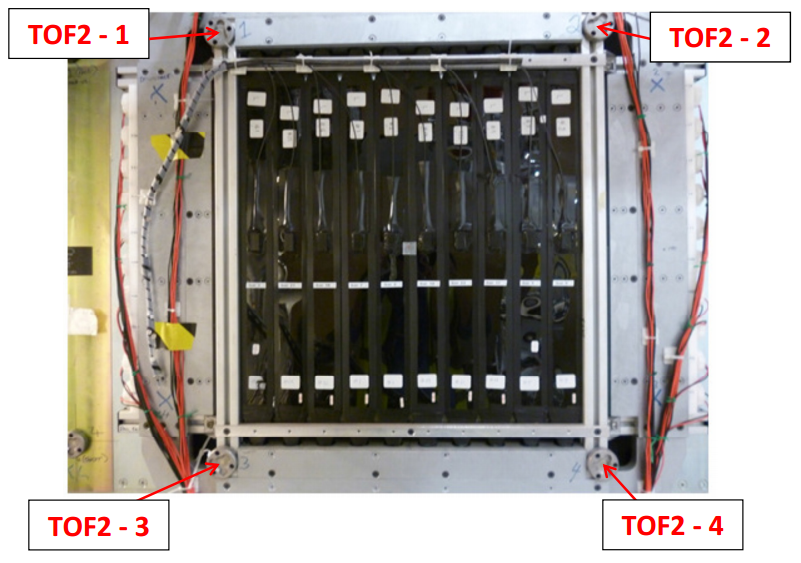
\includegraphics[width=\textwidth]{tof2_monuments.png}
		\caption{Picture of the TOF2 time-of-flight hodoscope and its four survey monuments labelled TOF2.1--2.4.}
		\label{fig:tof2_monuments}
	\end{minipage}
	\hfill
	\begin{minipage}[b]{.45\textwidth}
		\centering
		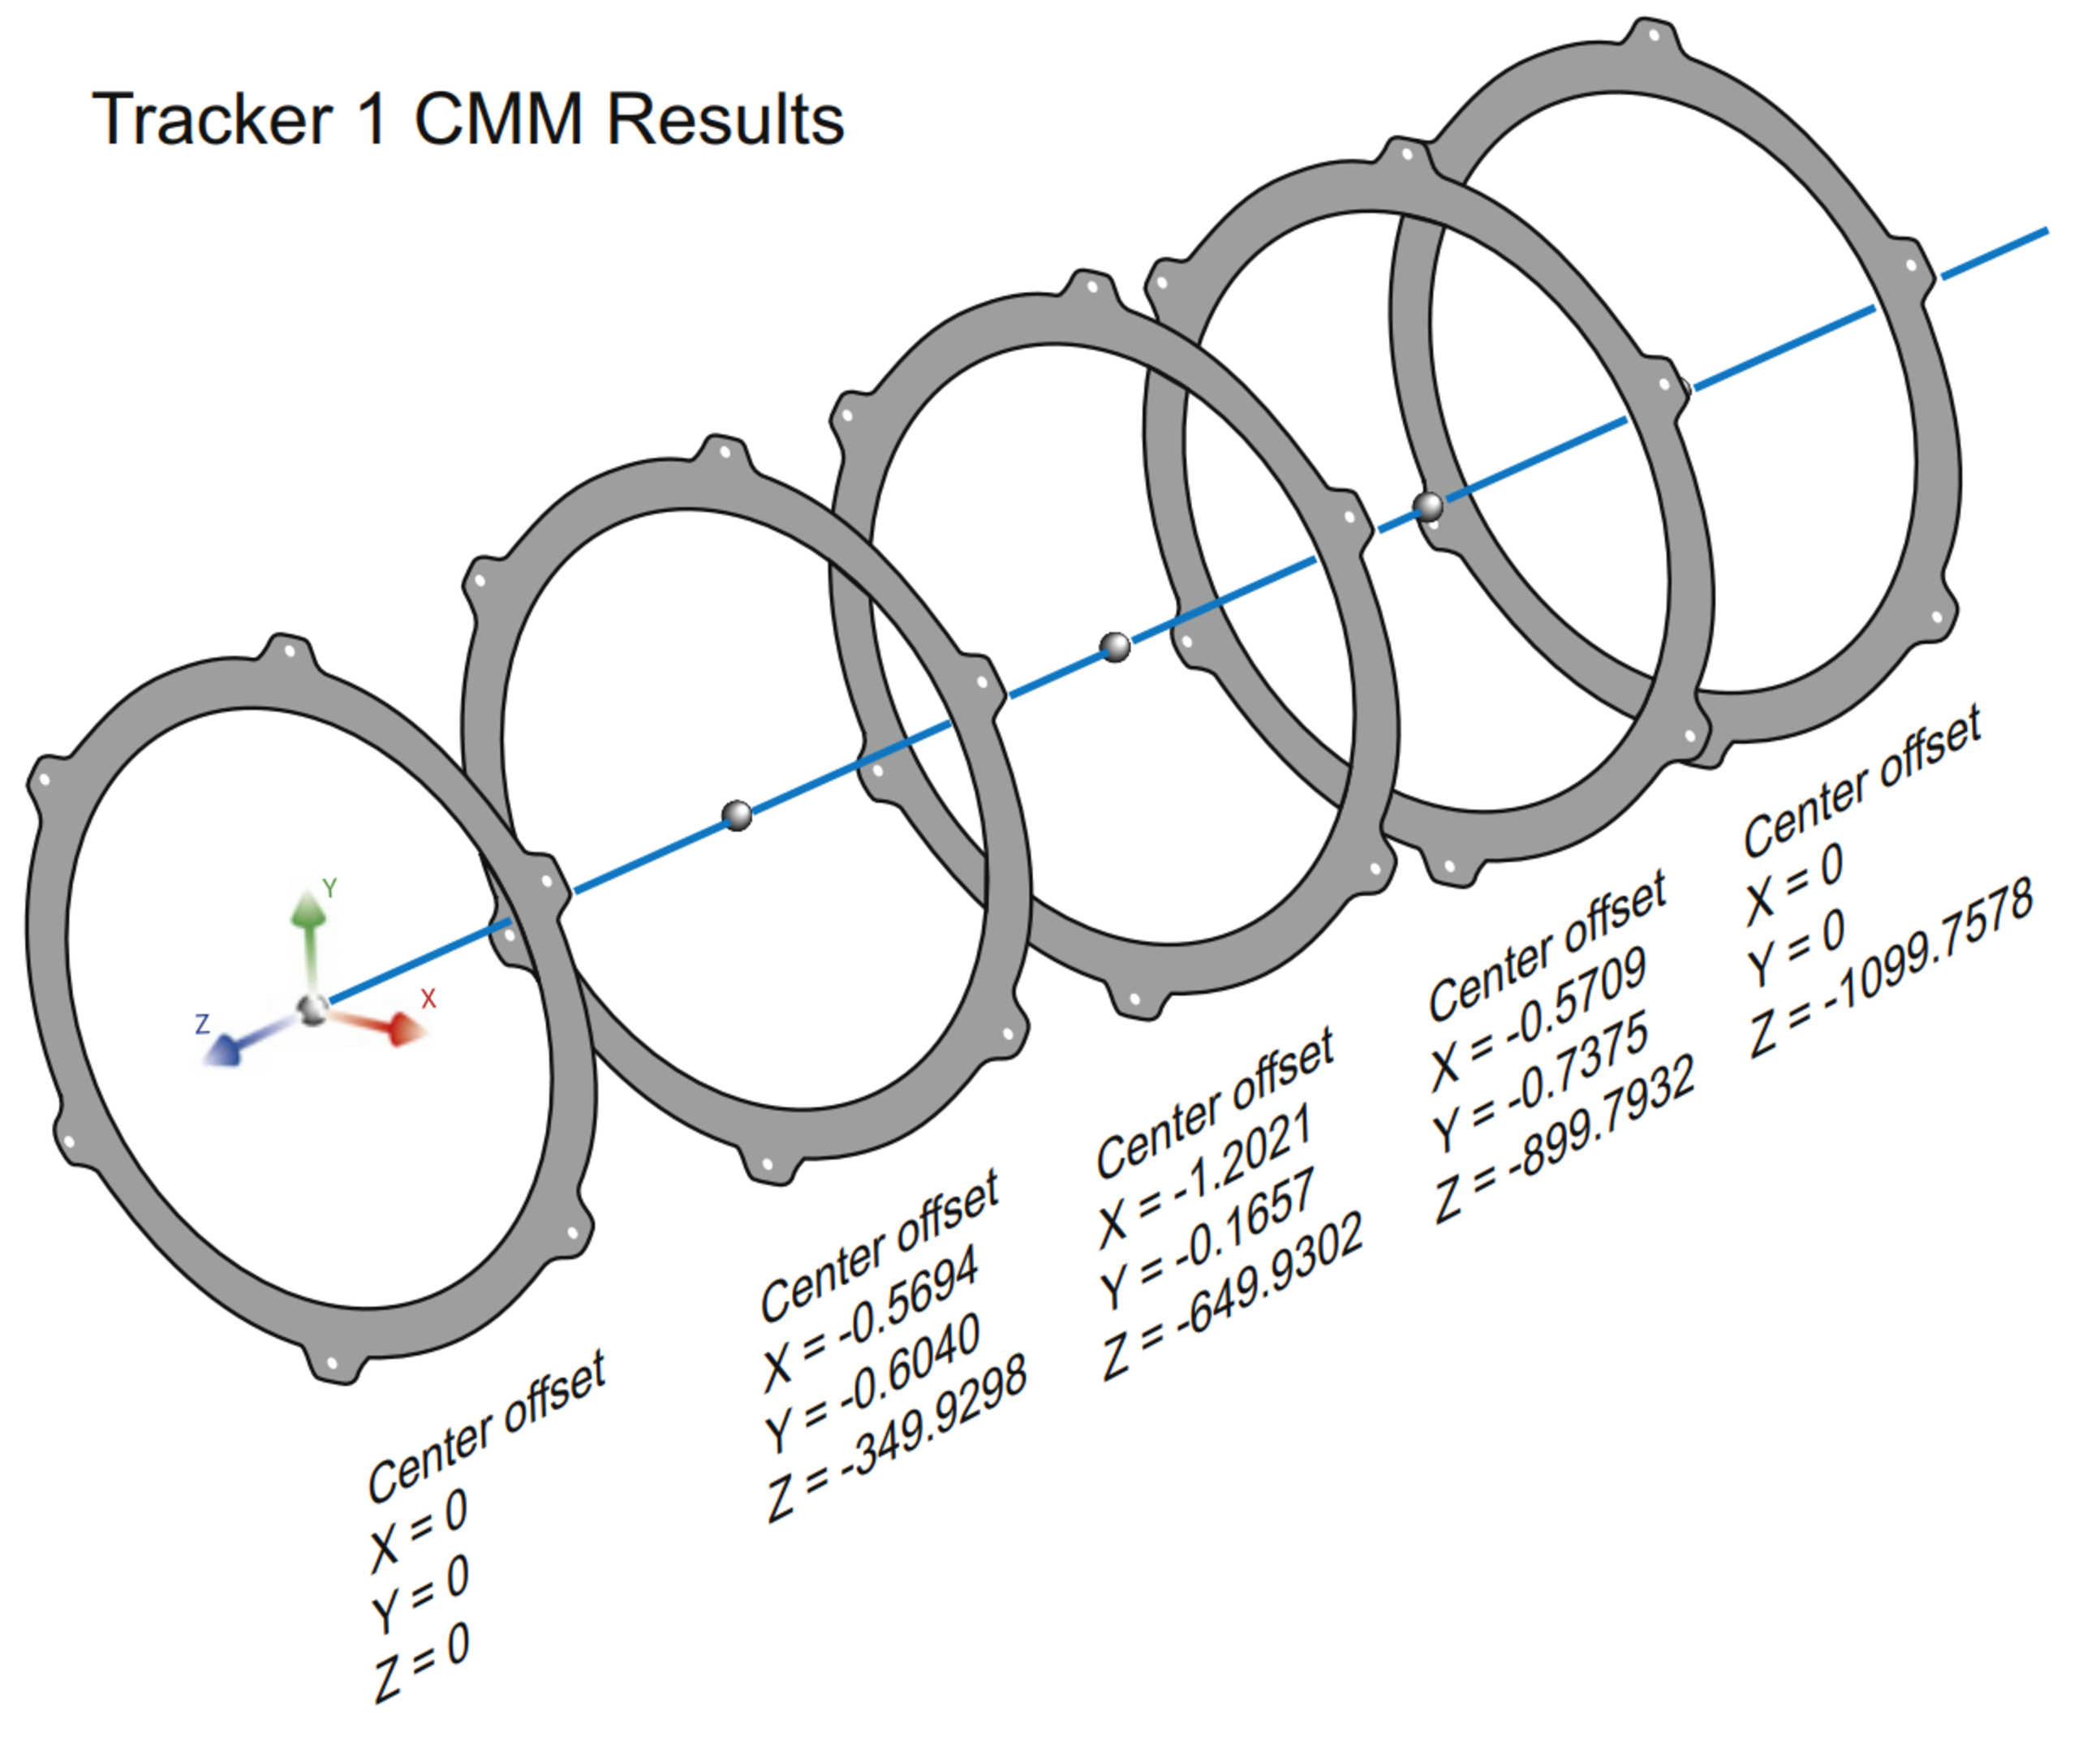
\includegraphics[width=\textwidth]{cmm_measurements.pdf}
		\caption{Disposition of the downstream tracker stations along with the CMM measurements of their position with respect to the reference axis.}
		\label{fig:cmm_measurements}
	\end{minipage}
\end{figure}

Before being placed inside the magnets, each tracker was surveyed independently using a coordinate-measuring machine (CMM). This ensures that the position of the five stations is well known within each tracker with respect to the end plate. Figure~\ref{fig:cmm_measurements} shows the disposition of the stations in the downstream scintillating fibre tracker and their position as measured by the CMM. The reference position is the axis that joins the centre of station 1 to the centre of station 5. The positions of stations 1 to 3 are measured with respect to that axis. The beam can be used to check the tracker station alignment.

Special care is taken during the installation of the trackers within the magnet bores. The installation platform is adjustable to enable the tracker to be aligned with the bore of the solenoid. The tracker sits on four adjustable feet, two at each end. The adjustable feet are used to align the tracker with the magnetic axis of the solenoid. Once this has been done, the location bracket is fitted. The location bracket locks the tracker in its longitudinal and azimuthal positions.

\subsection{Analysis method}
\label{SubSect:DA_Analysis}

The position of tracker $t=u,d$ in global coordinates is entirely defined by the location of its centre $(x_\mathrm{T},y_\mathrm{T},z_\mathrm{T})$ and a set of Tait-Bryan angles $(\alpha_T,\beta_T,\gamma_T)$. The $z$ axis is oriented along the beam line and points downstream, the $y$ axis points upwards and the $x$ axis completes the right-handed coordinate system. The rotation about $x$, $\alpha_T$, is called pitch, about $y$, $\beta_T$, is called yaw and about $z$, $\gamma_T$, is called roll. For a straight track of local coordinates $(x_t,y_t,z_t)$ at the tracker centre, the global coordinates are reconstructed as
\begin{equation}
\begin{pmatrix}
\xi_t \\
\upsilon_t \\
\zeta_t  
\end{pmatrix} =
\begin{pmatrix}
x_t-\gamma_T y_t+\beta_T z_t+x_\mathrm{T} \\
y_t+\gamma_T x_t-\alpha_T z_t+y_\mathrm{T} \\
z_t-\beta_T x_t+\alpha_T y_t+z_\mathrm{T}
\end{pmatrix}\, .
\label{eq:rot_matrix}
\end{equation}
in the first order small angles approximation. The global gradients of the straight track thus read
\begin{equation}
\begin{gathered}
\xi'_t = \frac{d\xi_t}{d\zeta_t} = \frac{dx_t-\gamma_Tdy_t+\beta_Tdz_t}{dz_t\left(1-\beta_Tx'_t+\alpha_Ty'_t\right)} \simeq x'_t-\gamma_T y'_t +\beta_T, \\
\upsilon'_t = \frac{d\upsilon_t}{d\zeta_t} = \frac{dy_t+\gamma_Tdx_t-\alpha_Tdz_t}{dz_t\left(1-\beta_Tx'_t+\alpha_Ty'_t\right)} \simeq y'_t+\gamma_T x'_t -\alpha_T.
\end{gathered}
\label{eq:global_grad}
\end{equation}

There are six potential unknowns per tracker. Some simplifications can be made to lower the amount of unknowns. The $z_T$ coordinate of each tracker is known to great accuracy from the survey. It may also be shown that the roll of the trackers has negligible influence on the alignment and may be ignored~\cite{2018arXiv1805.06623T}. The beam-based detector alignment is critical to find the $(x_\mathrm{T}, y_\mathrm{T}, \alpha_\mathrm{T}, \beta_\mathrm{T})$ constants for each tracker.

The location of the TOFs is used as the reference for the tracker alignment. The line that joins the centre of TOF1 with the centre of TOF2 is chosen to be the reference axis. A deviation from this axis is considered as a misalignment of the trackers. Multiple scattering in the beam line does not allow to do the alignment on single particle basis but works for a larger sample of particles. The mean residual angles and positions of the trackers with respect to the TOF12 axis are an essential and powerful tool to infer the correction factors. Figure~\ref{fig:align_bl} shows the path of a single particle that scatters in the absorber module of the MICE experiment.

\begin{figure}
	\begin{center}
		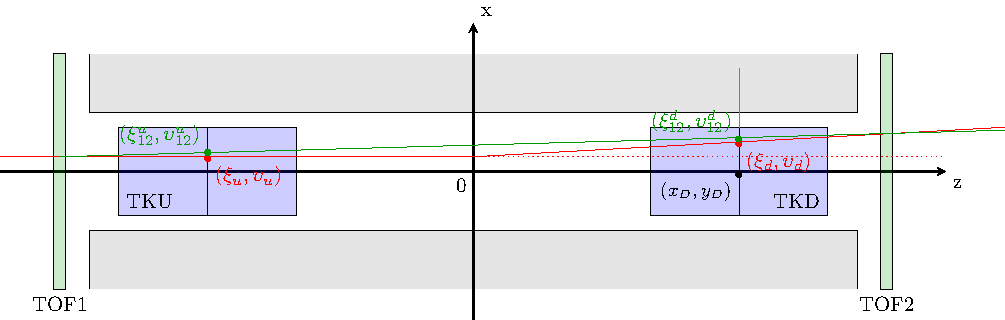
\includegraphics[width=0.95\textwidth]{alignment.pdf}
	\end{center}
	\caption{
		True path of a single particle track (red) and its path as reconstructed from the time-of-flight system (green). The position of the track at the tracker centres is represented by markers.
	}
	\label{Fig:AbsorberVessel:BdyPhoto}
\end{figure}

Each TOF provides a single space point in the global coordinate system $(\xi_i, \upsilon_i, \zeta_i)$ with $i$ the ID of the TOF. This position is assumed to be the true position with a large uncertainty due to the limited granularity of the detector ($\sigma_x\sim\sigma_y\sim17$\,mm). The gradients of the track between the two TOFs are reconstructed as:
\begin{equation}
\psi'_{12}=\frac{\psi_2-\psi_1}{\zeta_2-\zeta_1},\quad\psi=\xi,\upsilon.
\end{equation}
The extrapolated position of the TOF reference track in the centre of tracker $t=u,d$ is
\begin{equation}
\psi_{12}^t=\psi_1+\frac{\psi_2-\psi_1}{\zeta_2-\zeta_1}(\zeta_T-\zeta_1)=(1-\chi_T)\psi_1+\chi_T\psi_2,\quad\psi=\xi,\upsilon,
\end{equation}
with $\chi_\mathrm{T}=(\zeta_T-\zeta_1)/(\zeta_2-\zeta_1)$, the fractional distance from TOF1 to the tracker centre.

Tracker $t=u,d$ samples the particle track in five different stations $(x_t^j, y_t^j, z_t^j)$, with $j=1,\dots,5,$. This allows for the reconstruction of a straight track with gradients $x'_t$ (resp. $y'_t$) in the $xz$ (resp. $yz$) projection and its position at the centre, $(x_t, y_t, 0)$. No assumption is made on the prior position of the tracker and hence the coordinates and gradients are returned in local coordinates, i.e. assuming a tracker perfectly aligned with the beam axis, whose centre lies at $z=0$.

In global coordinates, on average, the track reconstructed between TOF1 and TOF2 should agree with the track reconstructed in either tracker, i.e. the mean residuals should be zero. Applying this reasoning to the unknown offset and angles yields the following system of four equations with four unknowns~\cite{2018arXiv1805.06623T}:
\begin{equation}
\left\{
\begin{array}{l}
\langle x'_t-\xi'_{12}\rangle = - \beta_T \\
\langle y'_t-\upsilon'_{12}\rangle = \alpha_T \\
\langle x_t-\xi_{12}^t\rangle = - x_T \\
\langle y_t-\upsilon_{12}^t\rangle = - y_T
\end{array}
\right. .
\label{eq:res}
\end{equation}
The measurement of four residual distributions per tracker yields the alignment constants.

The method described here assumes that the mean residuals can be measured with great accuracy and, more importantly, are unbiased. A bias in one of the residual distributions inevitably introduces a bias in the measurement of the corresponding alignment parameter, as they are directly proportional. The main source of bias is the scattering in the material between TOF1 and TOF2. If the beam is not perfectly centred, particles preferentially scrape out on one side of the magnet bore, anisotropically curbing a specific tail of the residual distribution. To nullify this effect, a fiducial cut is applied to the upstream sample. Only particles that are expected to be contained in the downstream tracker are included in the analysis~\cite{2018arXiv1805.06623T}.


% --------------------------------------- %
% ------------------DATA----------------- %
% --------------------------------------- %
\subsection{Alignment of a data sample}
\label{SubSect:DA_Data}
Data is recorded with the superconducting magnetic channel of the experiment turned off, i.e. with tracks going in a straight line from TOF1 to the beam dump. High momentum beams are used in order to reduce the RMS scattering angle and maximize transmission. The settings used correspond to `pion' beams of positive polarity to maximize statistics. The beams exhibit a variety of distributions in the beam line.  An agreement between the independent fits guarantees an unbiased measurement of the alignment constants.

Provided with the unbiased sample produced as described in section\,\ref{SubSect:DA_Analysis}, each track yields a set of global gradients between TOF1 and TOF2, $\xi'_{12}$ and $\upsilon'_{12}$, and global extrapolated positions at the tracker centres, $\xi_{12}^t$ and $\upsilon_{12}^t$. It also records the position of the track at the centre of the trackers in local coordinates, $x_t$ and $y_t$, and its local gradients, $x'_t$ and $y'_t$. The residual distributions necessary to measure the left hand side of equations\,\ref{eq:res} are produced in order to measure the eight alignment parameters. Figure~\ref{fig:resyp} shows the gradient residuals between $y'_u$ and $\upsilon'_{12}$ for run 9367. The mean residual yields the the pitch of the upstream tracker, $\alpha_U$.

\begin{figure} [!htb]
	\begin{minipage}[b]{.48\textwidth}
		\centering
		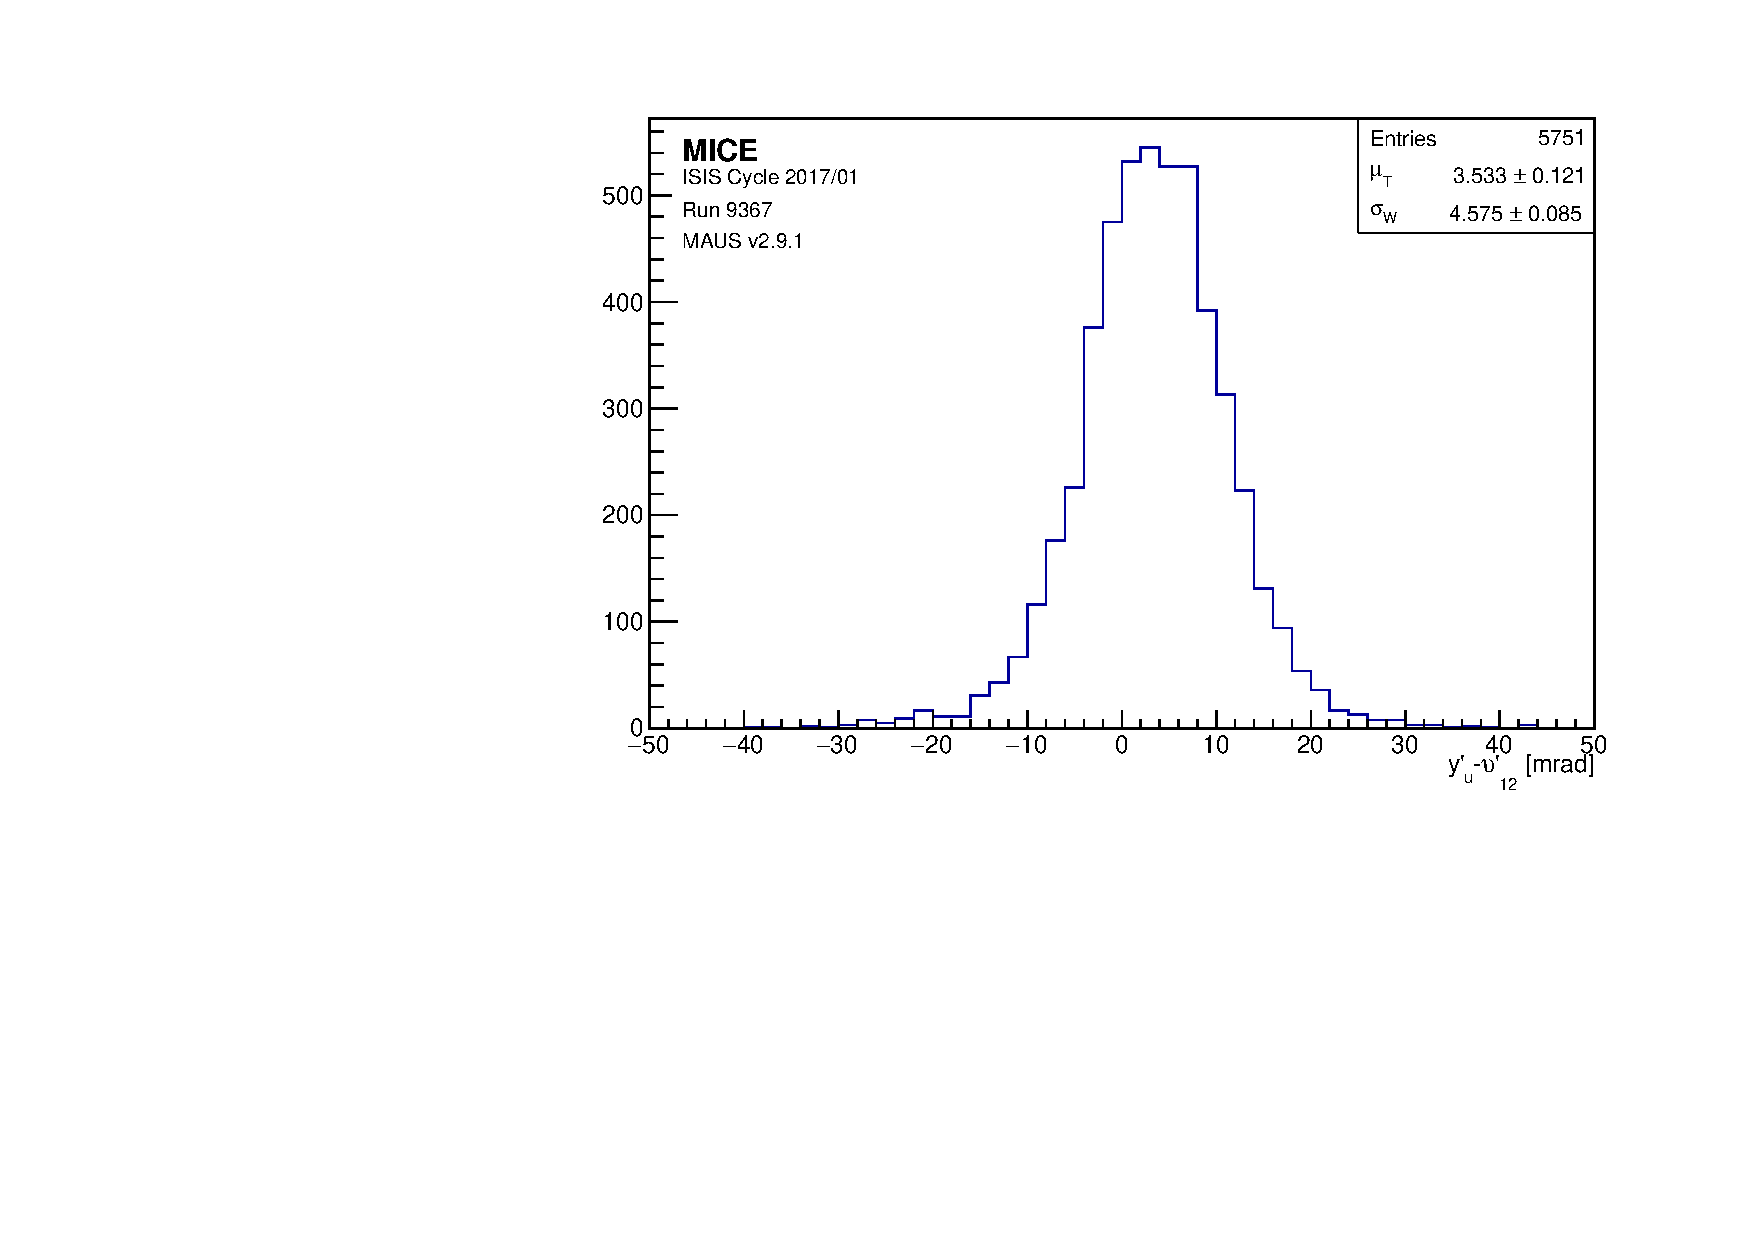
\includegraphics[width=\textwidth]{tku_resyp.pdf}
		\caption{Residuals distribution between the pitch gradients measured locally in TKU, $y'_u$, and globally between TOF1 and TOF2, $\upsilon'_{12}$.}
		\label{fig:resyp}
	\end{minipage}
	\hfill
	\begin{minipage}[b]{.48\textwidth}
		\centering
		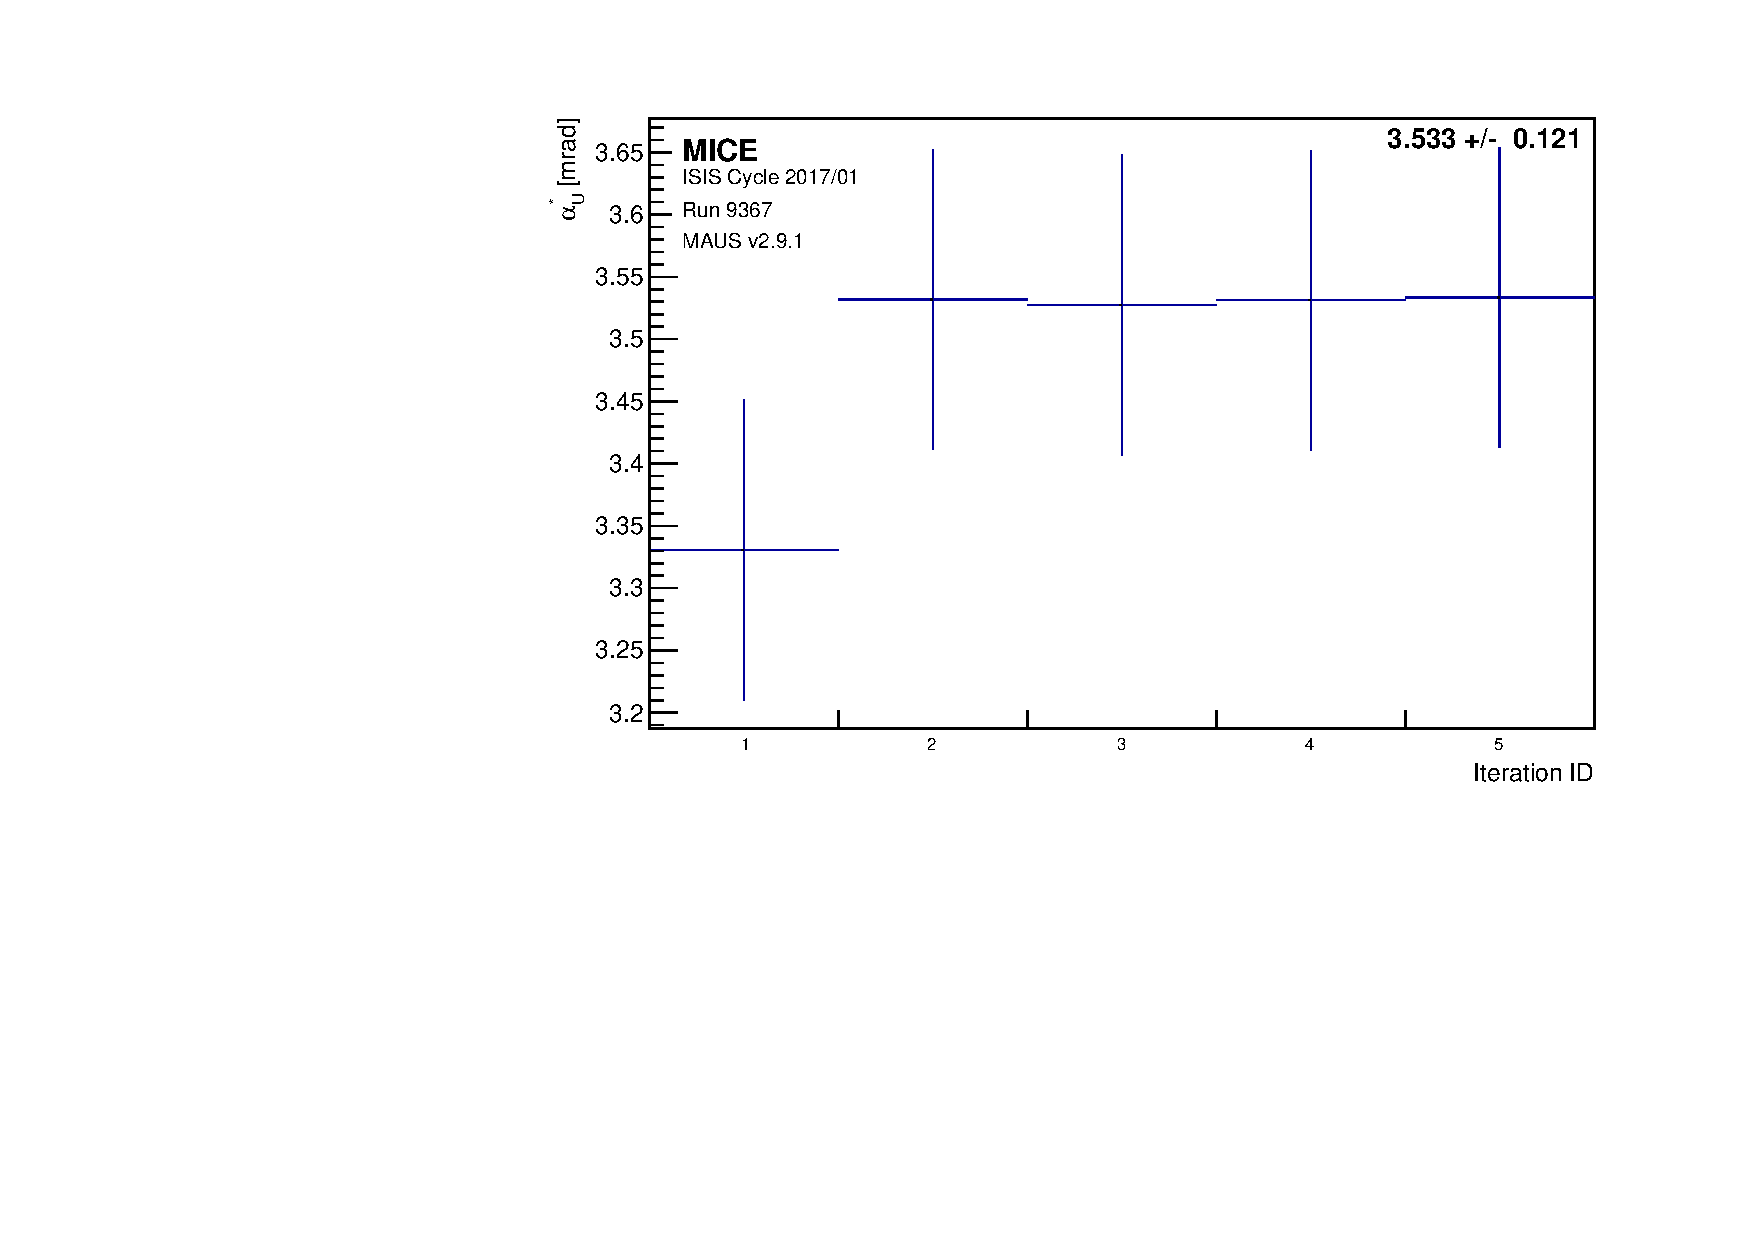
\includegraphics[width=\textwidth]{tku_optalpha.pdf}
		\caption{Evolution of the optimal value of the pitch angle in TKU, $\alpha_U^*$, for different number of iterations of the fitting algorithm.}
		\label{fig:optalpha}
	\end{minipage}
\end{figure}

To ensure the best possible fit to the tracker parameters, the algorithm is applied multiple times. The first estimate of $x_T,y_T,\alpha_T,\beta_T$ is used as an input to the sample selection part of the algorithm. The process is repeated until the alignment constants converge. Figure~\ref{fig:optalpha} shows the evolution of the optimal upstream tracker pitch, $\alpha_U^
*$, over five iterations for run 9367.

Each data set was processed independently with the algorithm. Figure~\ref{fig:runtorun} compiles the alignment parameters measured for each run. The measurements are in good agreement with one another and show no significant discrepancy. The constant fit $\chi^2/\text{ndf}$ is close to unity for each fit, which indicates that there are no significant additional source of uncertainty. The optimal parameters are summarised in table\,\ref{tab:201701_constants}.

\begin{table}[h!]
	\centering
		\begin{tabular}{l|c|c|c|c}
			& x [mm] & y [mm] & $\alpha$ [mrad] & $\beta$ [mrad] \\
			\hline
			TKU & $-0.032\pm0.094$ & $-1.538\pm0.095$ & $3.382\pm0.030$ & $0.412\pm0.029$ \\
			TKD & $-2.958\pm0.095$ & $2.921\pm0.096$ & $-0.036\pm0.030$ & $1.333\pm0.030$
		\end{tabular}
	\caption{Summary table of the optimal alignment constants measured in the high-momentum straight-track data acquired during the 2017/01 ISIS user cycle.}
	\label{tab:201701_constants}
\end{table}

\begin{figure} [!htb]
	\centering
	\begin{minipage}[b]{.49\textwidth}
		\centering
		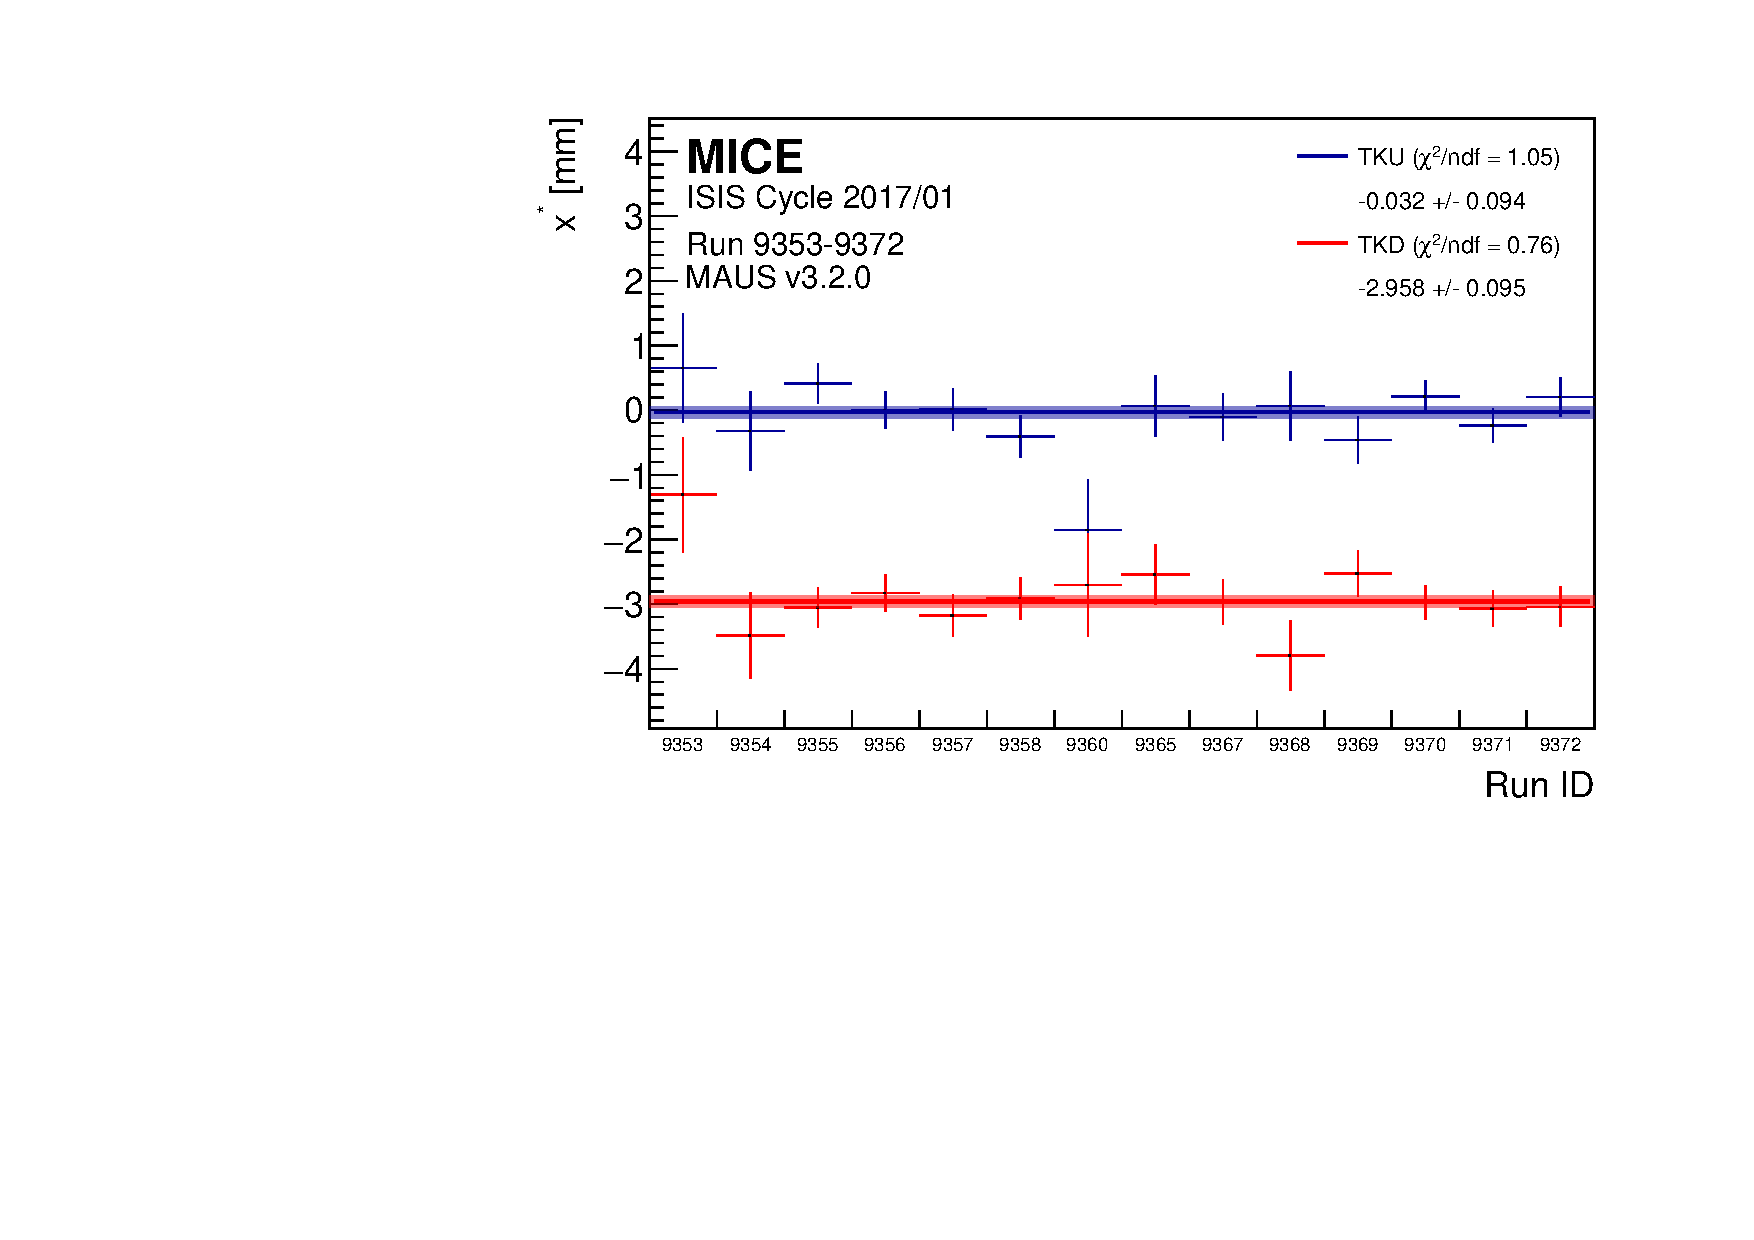
\includegraphics[width=\textwidth]{data_final/x_bestfit.pdf}
	\end{minipage}
	\hfill
	\begin{minipage}[b]{.49\textwidth}
		\centering
		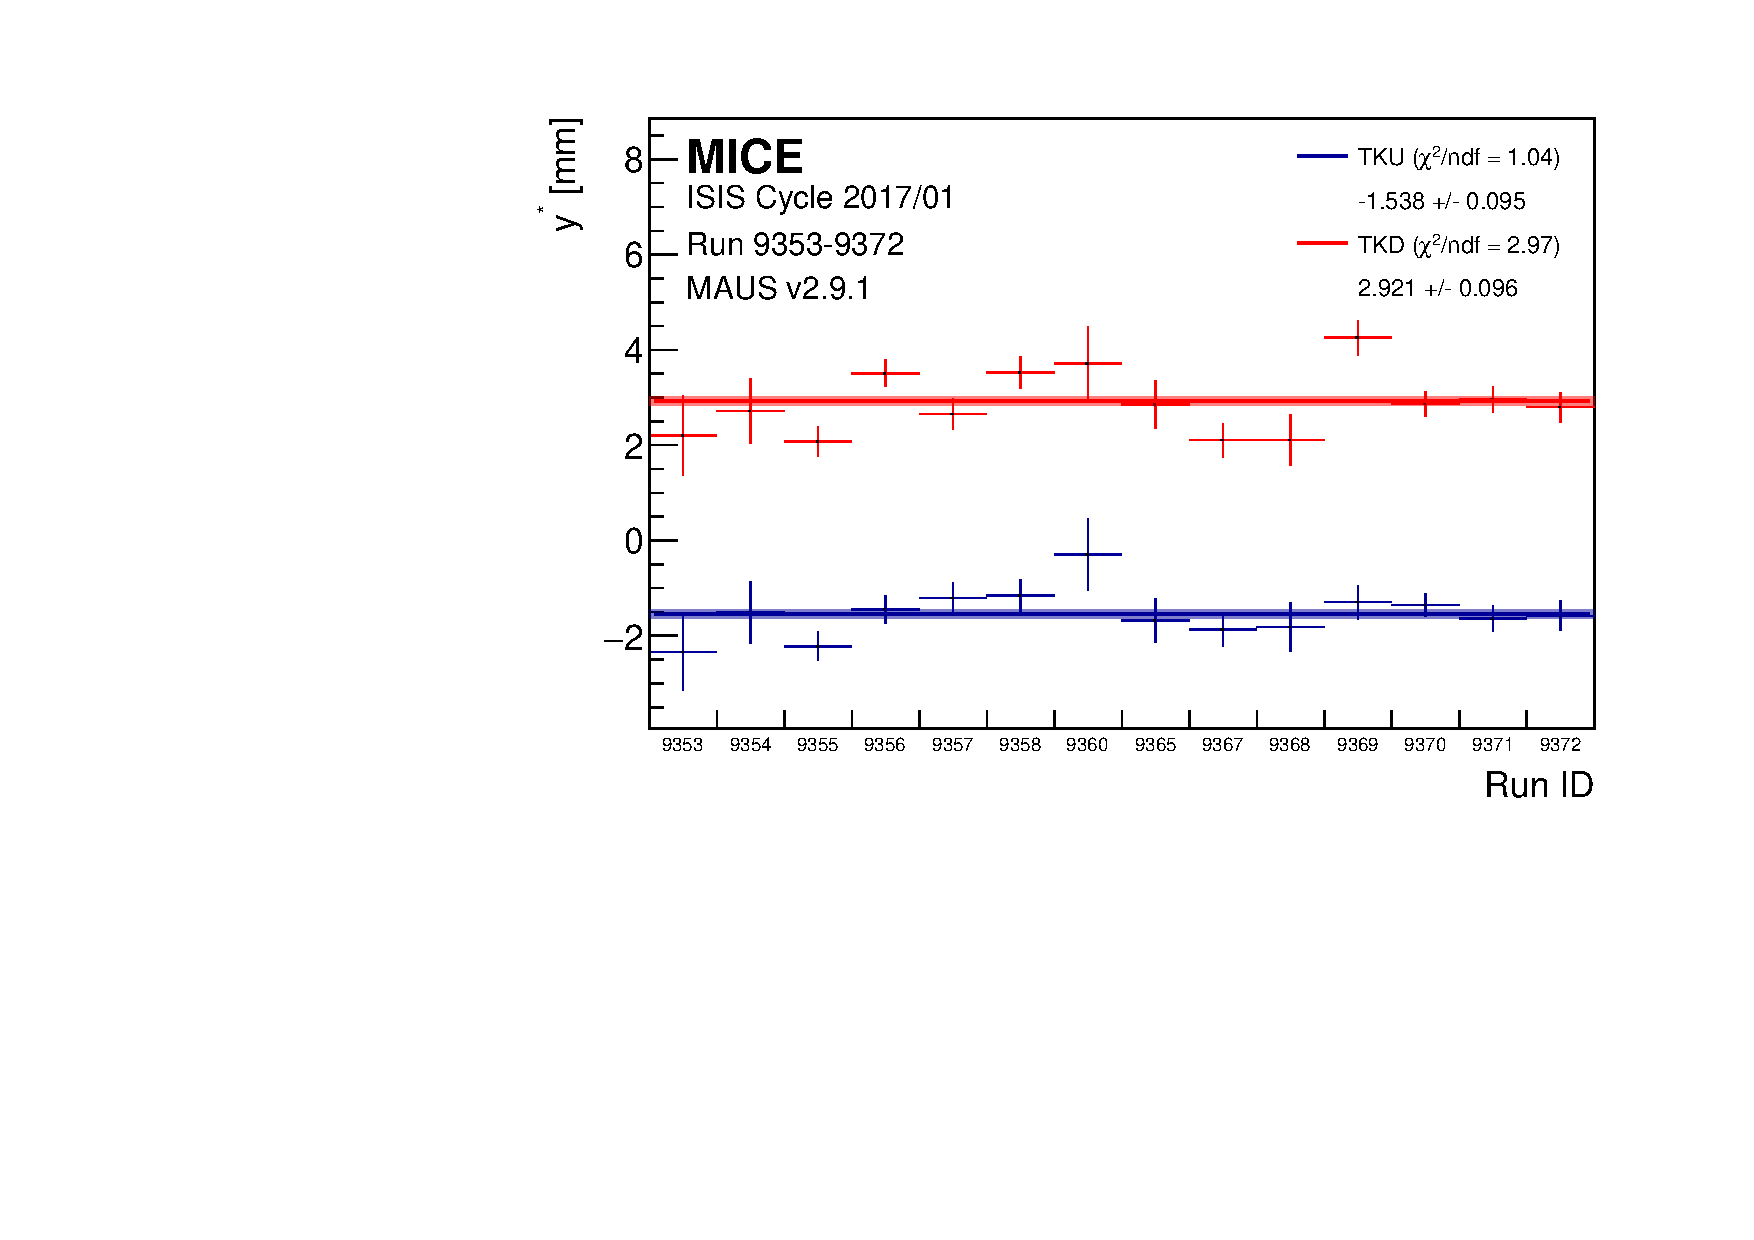
\includegraphics[width=\textwidth]{data_final/y_bestfit.pdf}
	\end{minipage}
	
	\begin{minipage}[b]{.49\textwidth}
		\centering
		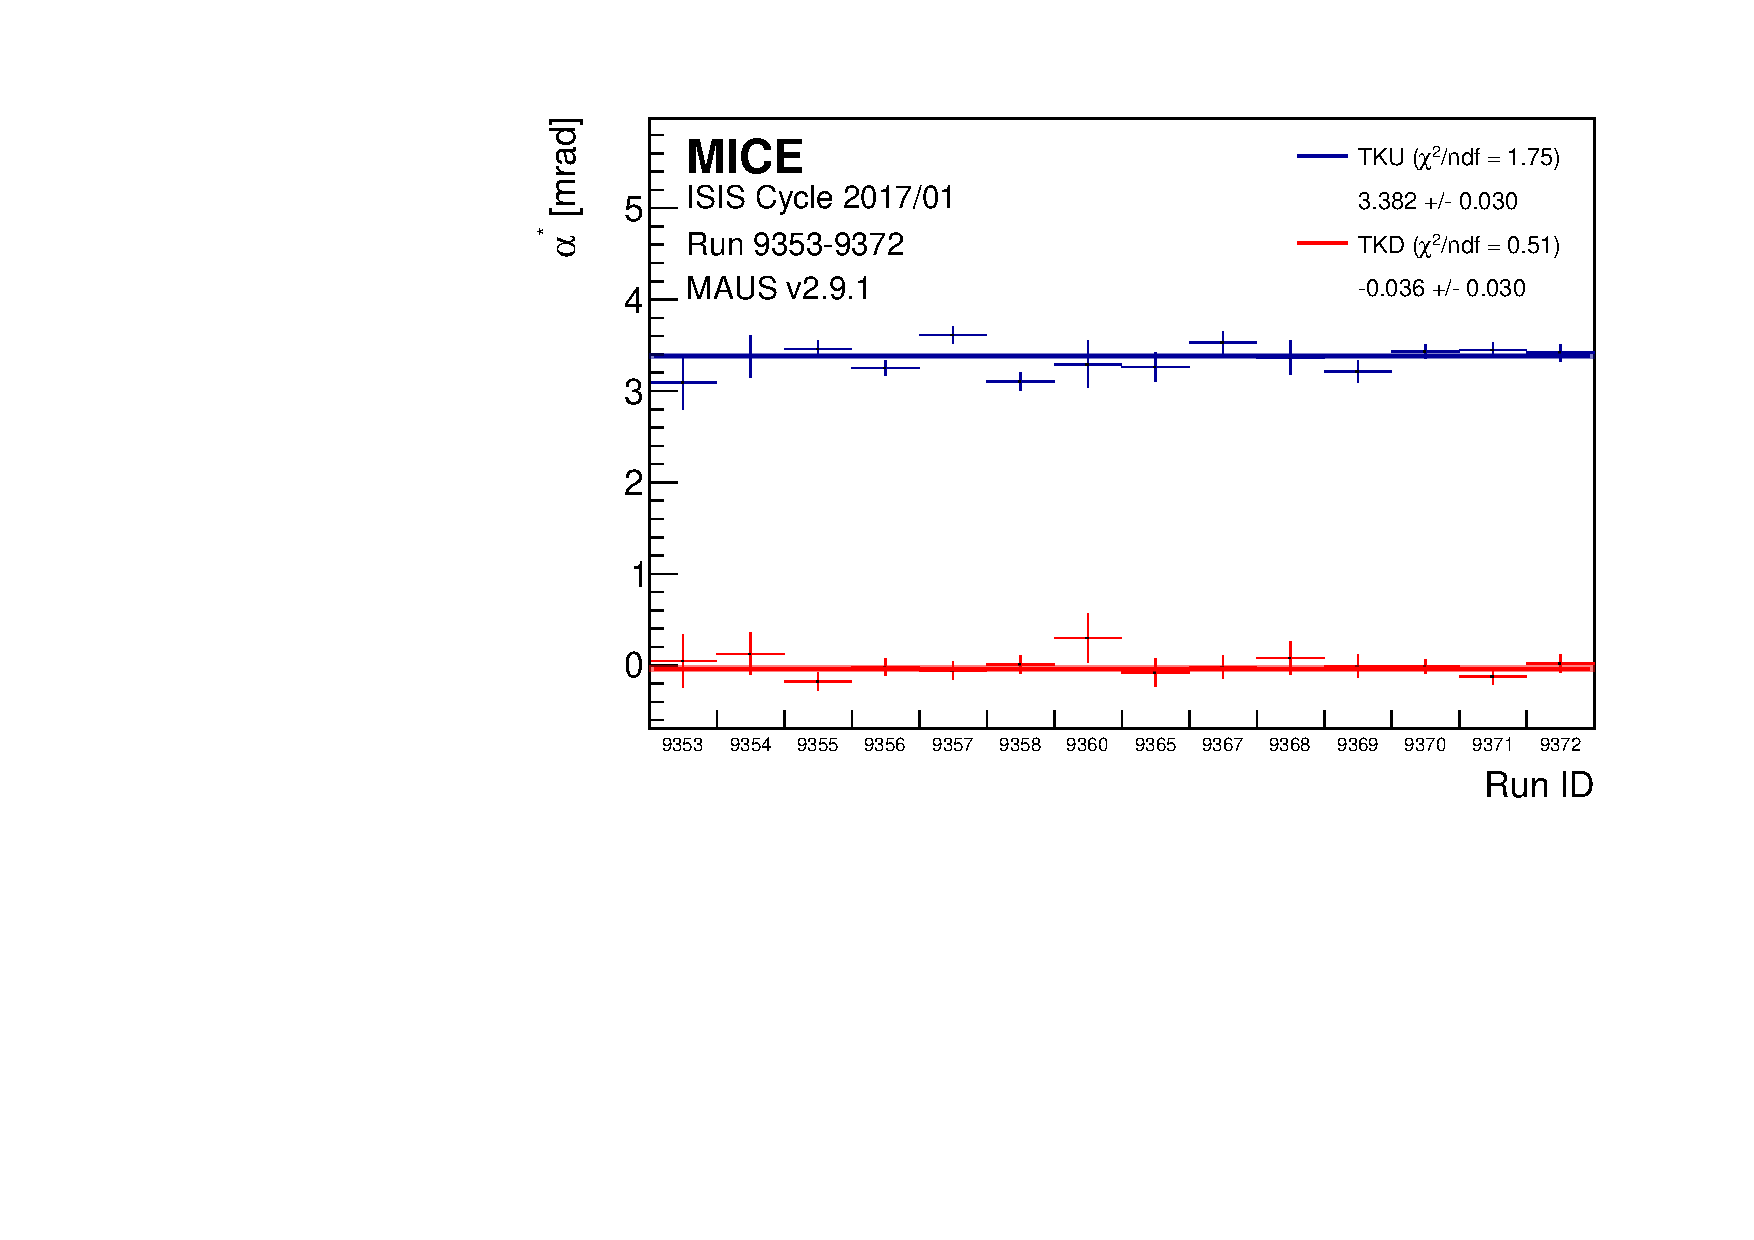
\includegraphics[width=\textwidth]{data_final/alpha_bestfit.pdf}
	\end{minipage}
	\hfill
	\begin{minipage}[b]{.49\textwidth}
		\centering
		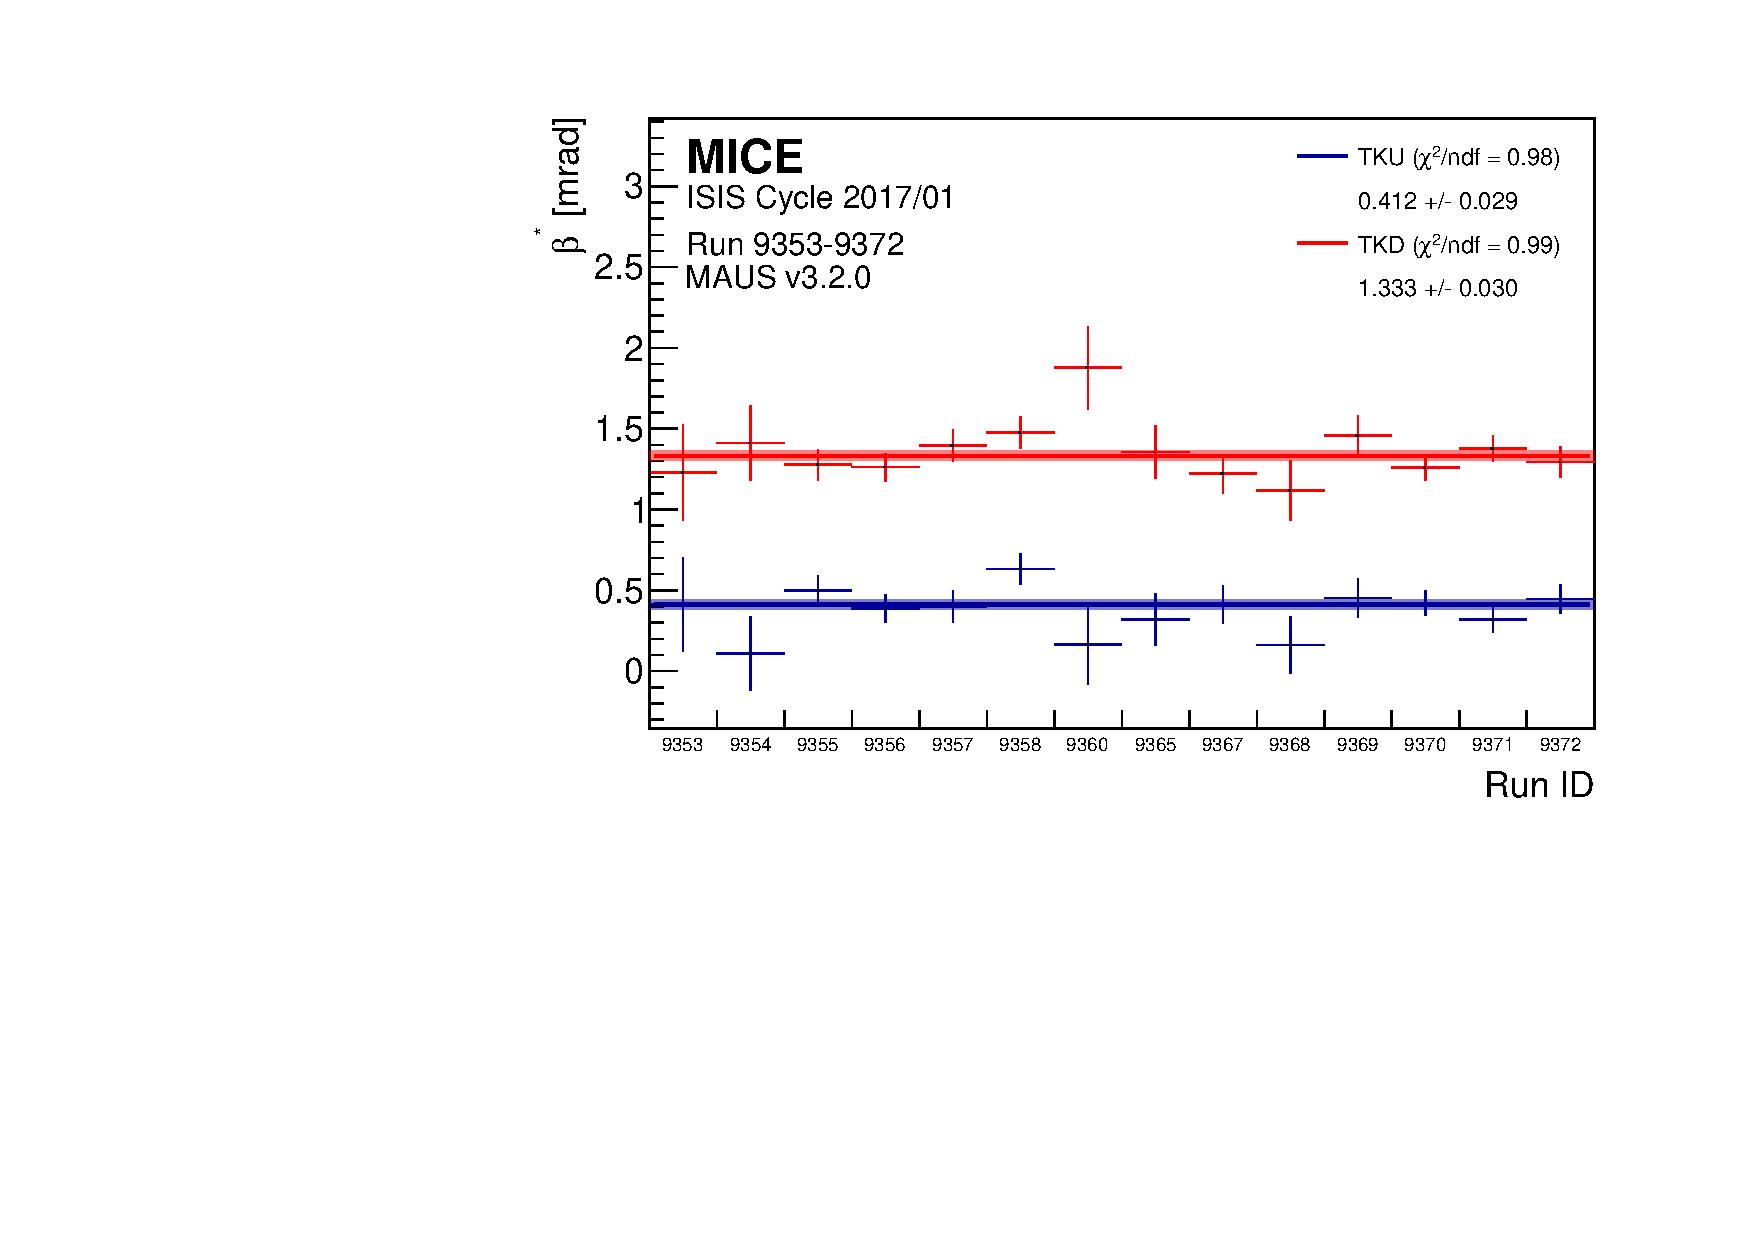
\includegraphics[width=\textwidth]{data_final/beta_bestfit.pdf}
	\end{minipage}
	\caption{Consistency of the alignment algorithm across runs acquired during the 2017/01 ISIS user cycle.}
	\label{fig:runtorun}
\end{figure}

\subsection{Propagation}
\label{SubSect:DA_Propagation}
The fitted parameters are used to yield the global track coordinates at the tracker $t=u,d$ centres, $(\xi_t,\upsilon_t,\zeta_t)$, through equation~\ref{eq:rot_matrix} and the global gradients $\xi'_t,\upsilon'_t$ through equation~\ref{eq:global_grad}. A corrected global track is propagated in an adjacent detector module $M$ at $\zeta_m$ through
\begin{equation}
\psi_t^m=\psi_t+\psi'_t(\zeta_m-\zeta_t),\,\psi=\xi,\upsilon.
\end{equation}

Provided exact corrections, a detector module $M$ that measures a global position $(\xi_m,\upsilon_m,\zeta_m)$ verifies
\begin{equation}
\left\{
\begin{array}{l}
\langle \psi_m-\psi_t^m\rangle=0 \\
\langle \psi'_m-\psi'_t\rangle=0
\end{array}
\right.,\,\psi=\xi,\upsilon.
\end{equation}

As a consistency check, the tracks are first propagated between the two trackers. The results are shown in figure~\ref{fig:tracker_residuals}. The top left and right distributions show the residuals between the TKU and TKD tracks at the centre of the downstream tracker and at the level of the absorber, respectively. The bottom two histograms show the agreement between the angles measured upstream and downstream. The azimuthal angle residuals show consistency between the roll of the two trackers.

\begin{figure} [!htb]
	\centering
	\begin{minipage}[b]{.475\textwidth}
		\centering
		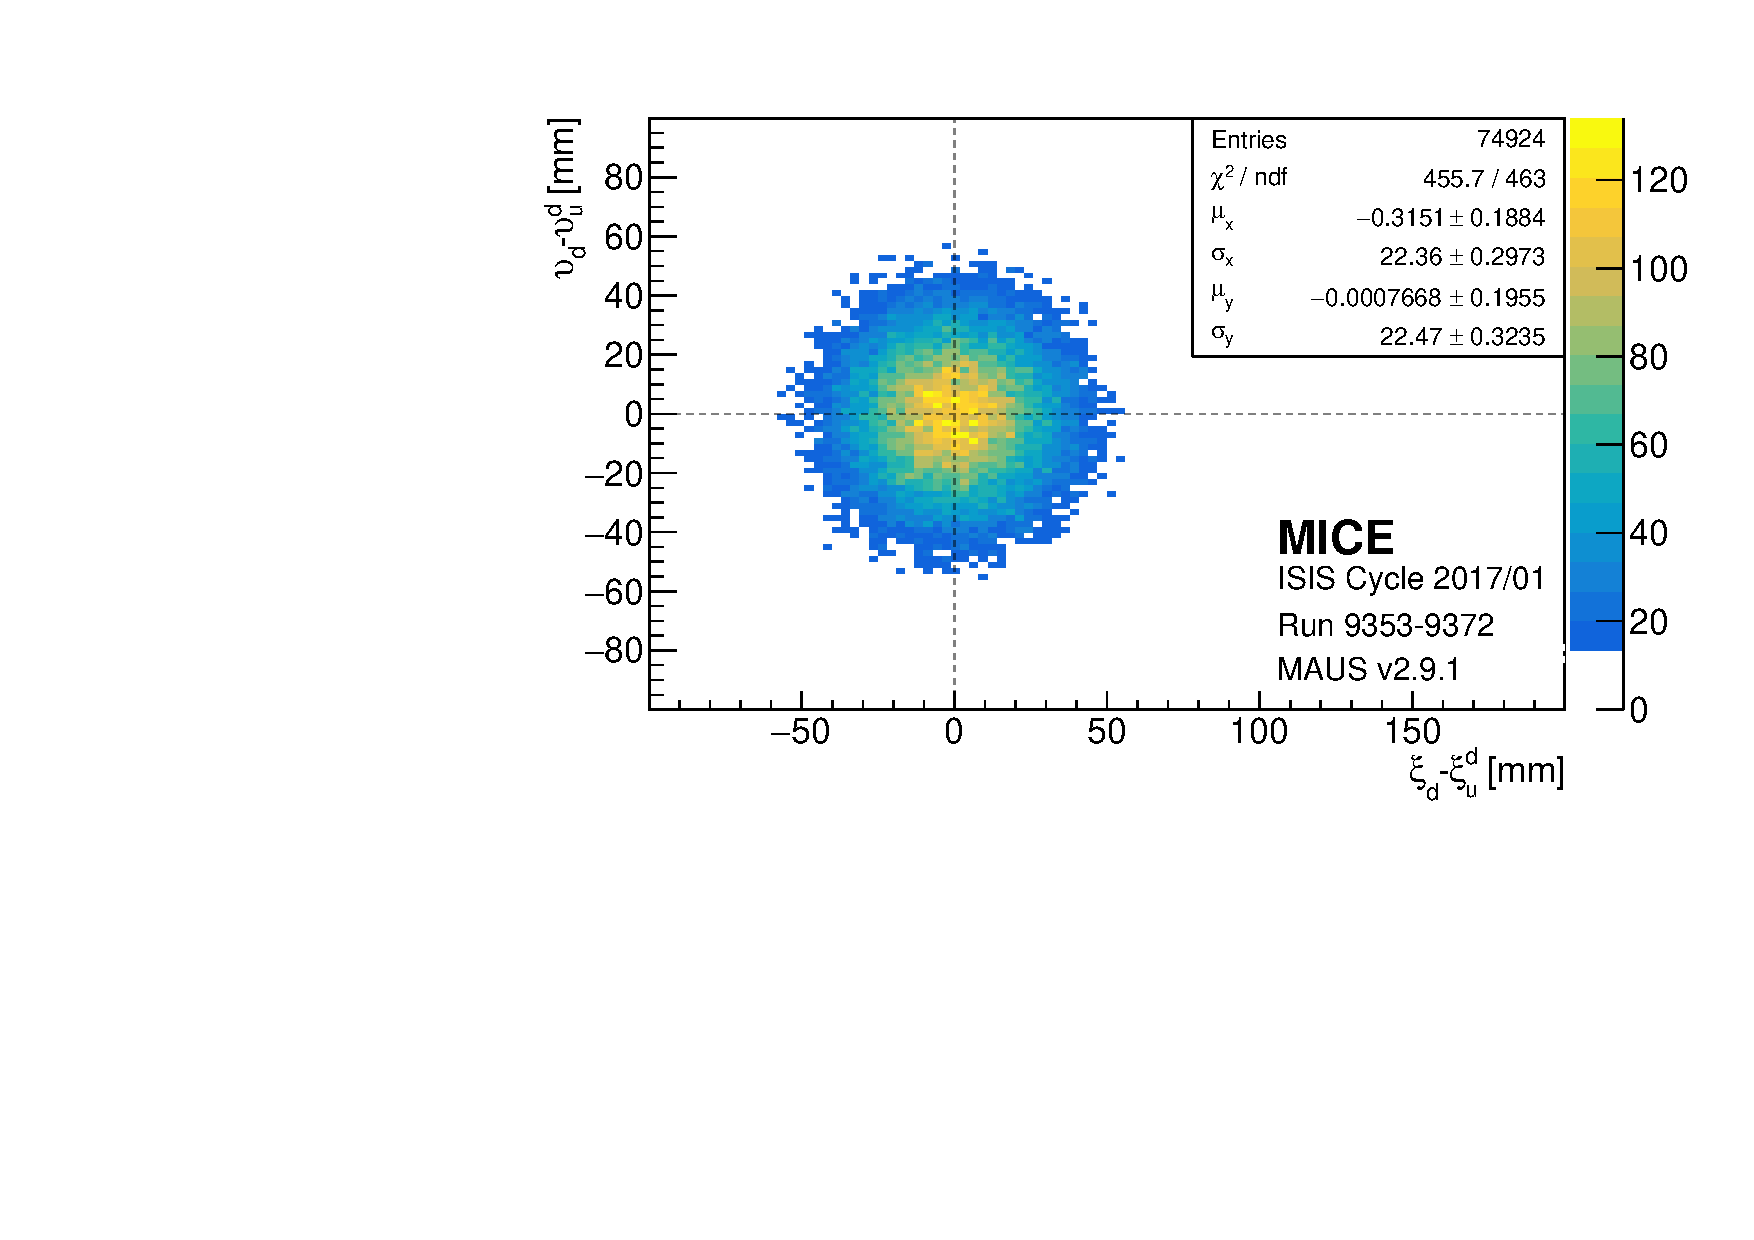
\includegraphics[width=\textwidth]{data_test/tkd_xy_res.pdf}
	\end{minipage}
	\hfill
	\begin{minipage}[b]{.475\textwidth}
		\centering
		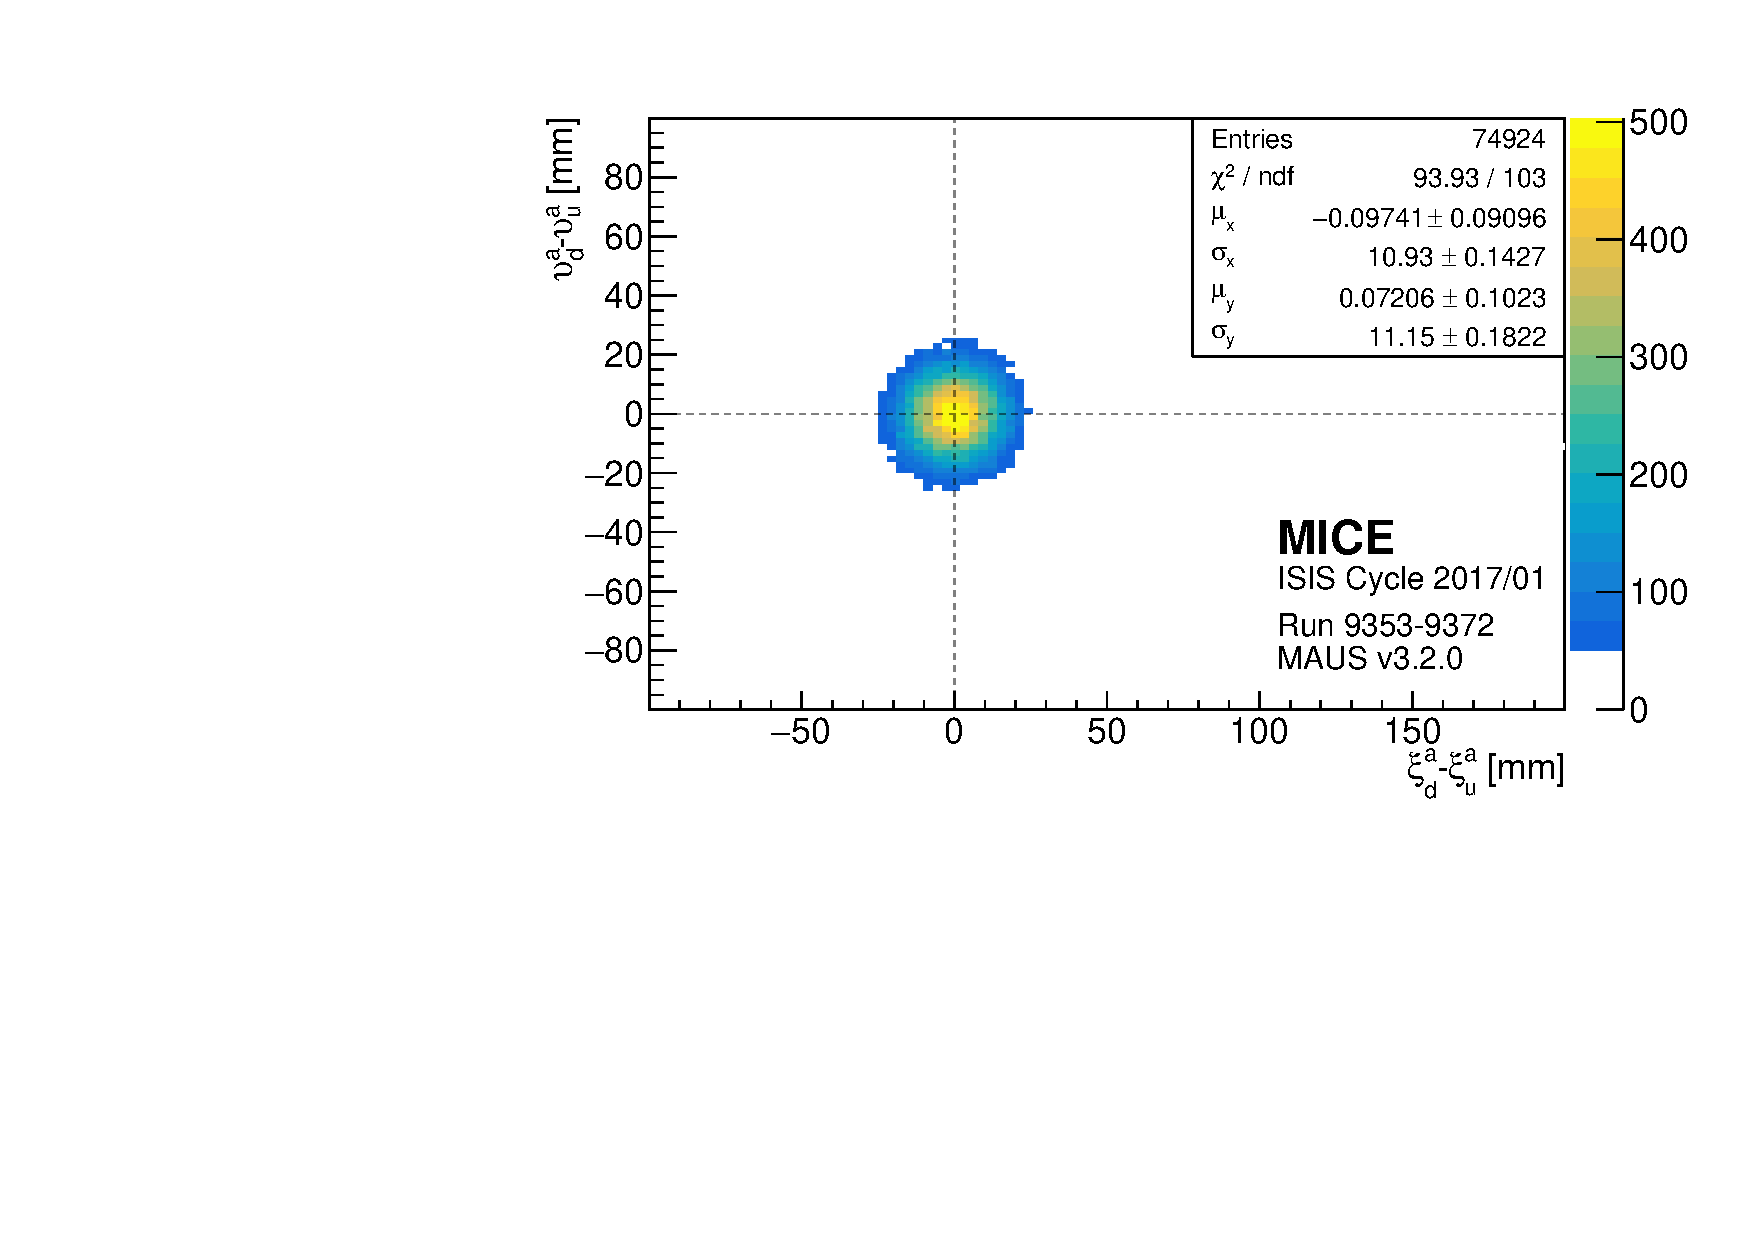
\includegraphics[width=\textwidth]{data_test/abs_xy_res.pdf}
	\end{minipage}
	
	\begin{minipage}[b]{.475\textwidth}
		\centering
		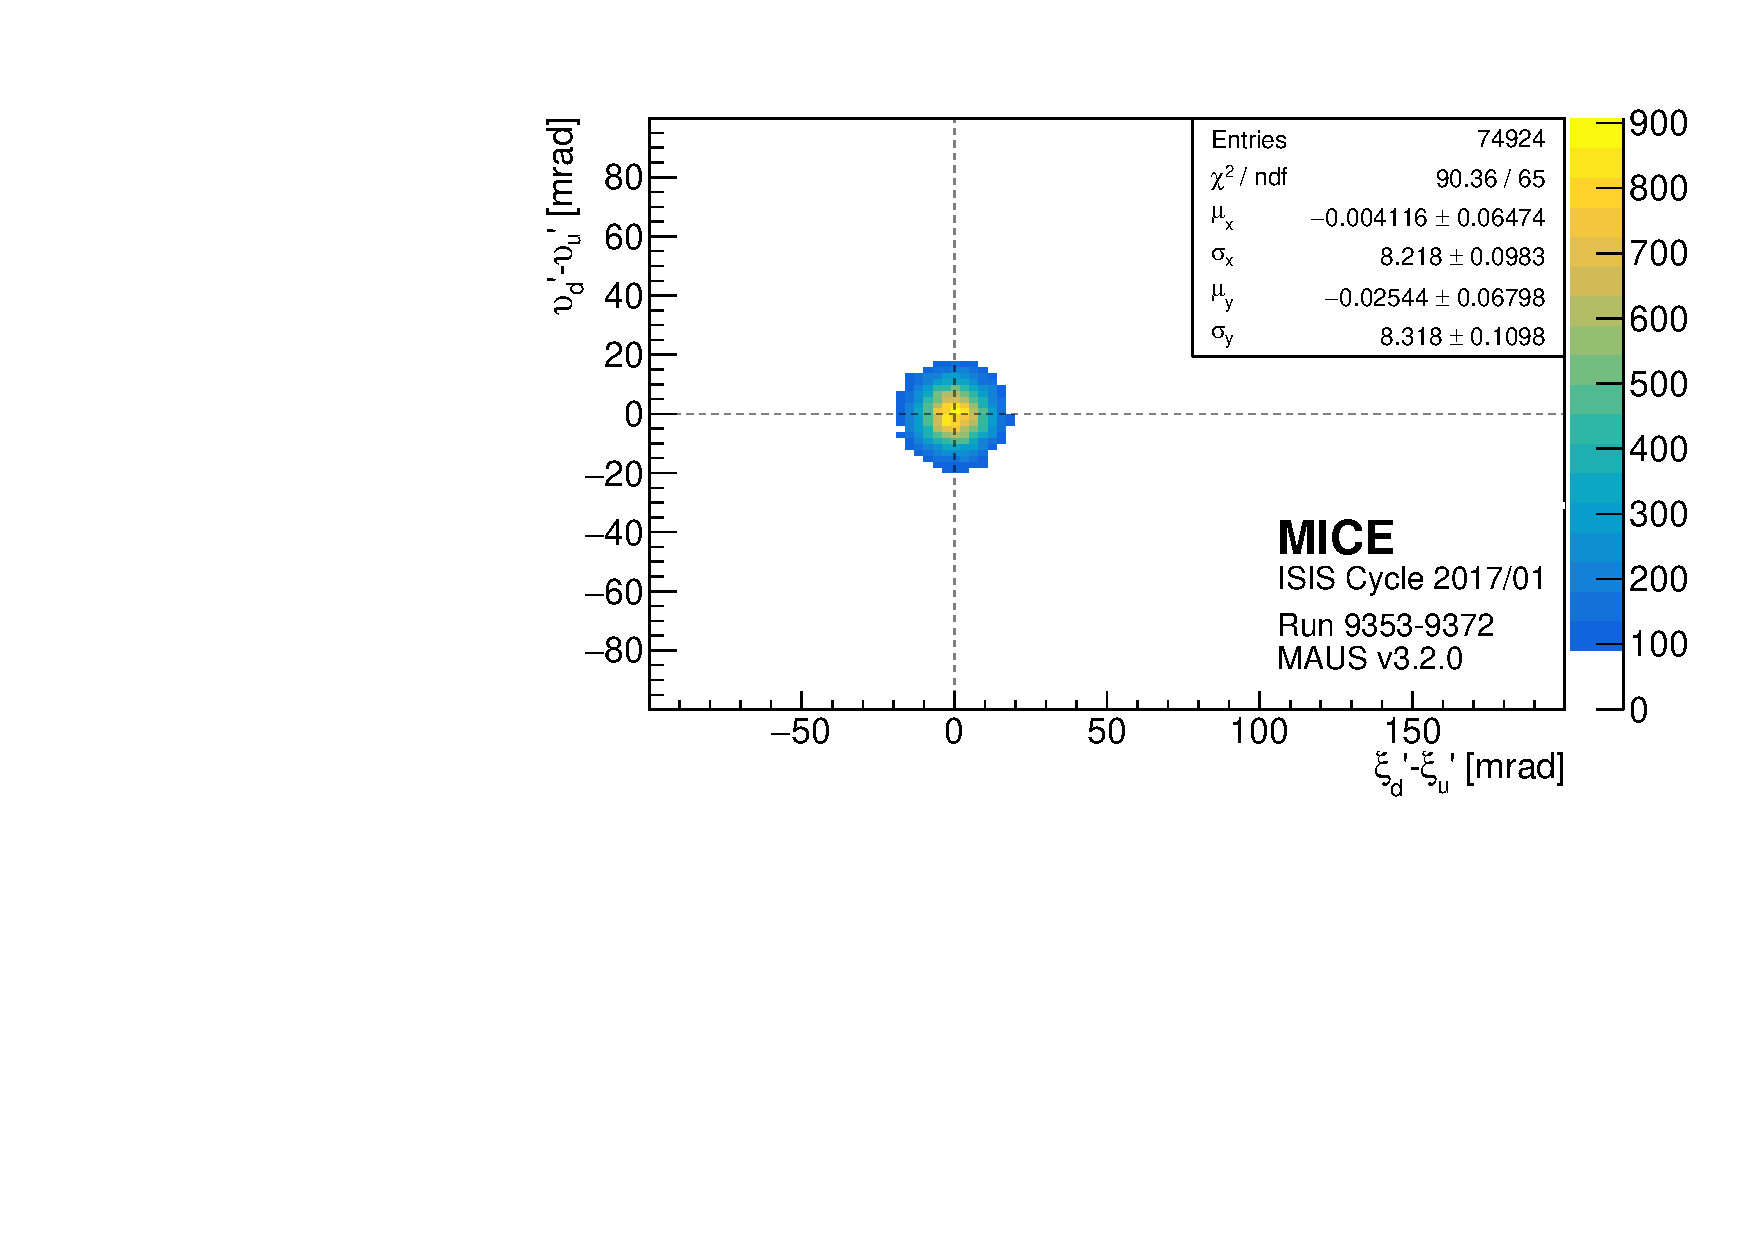
\includegraphics[width=\textwidth]{data_test/tkd_xpyp_res.pdf}
	\end{minipage}
	\hfill
	\begin{minipage}[b]{.475\textwidth}
		\centering
		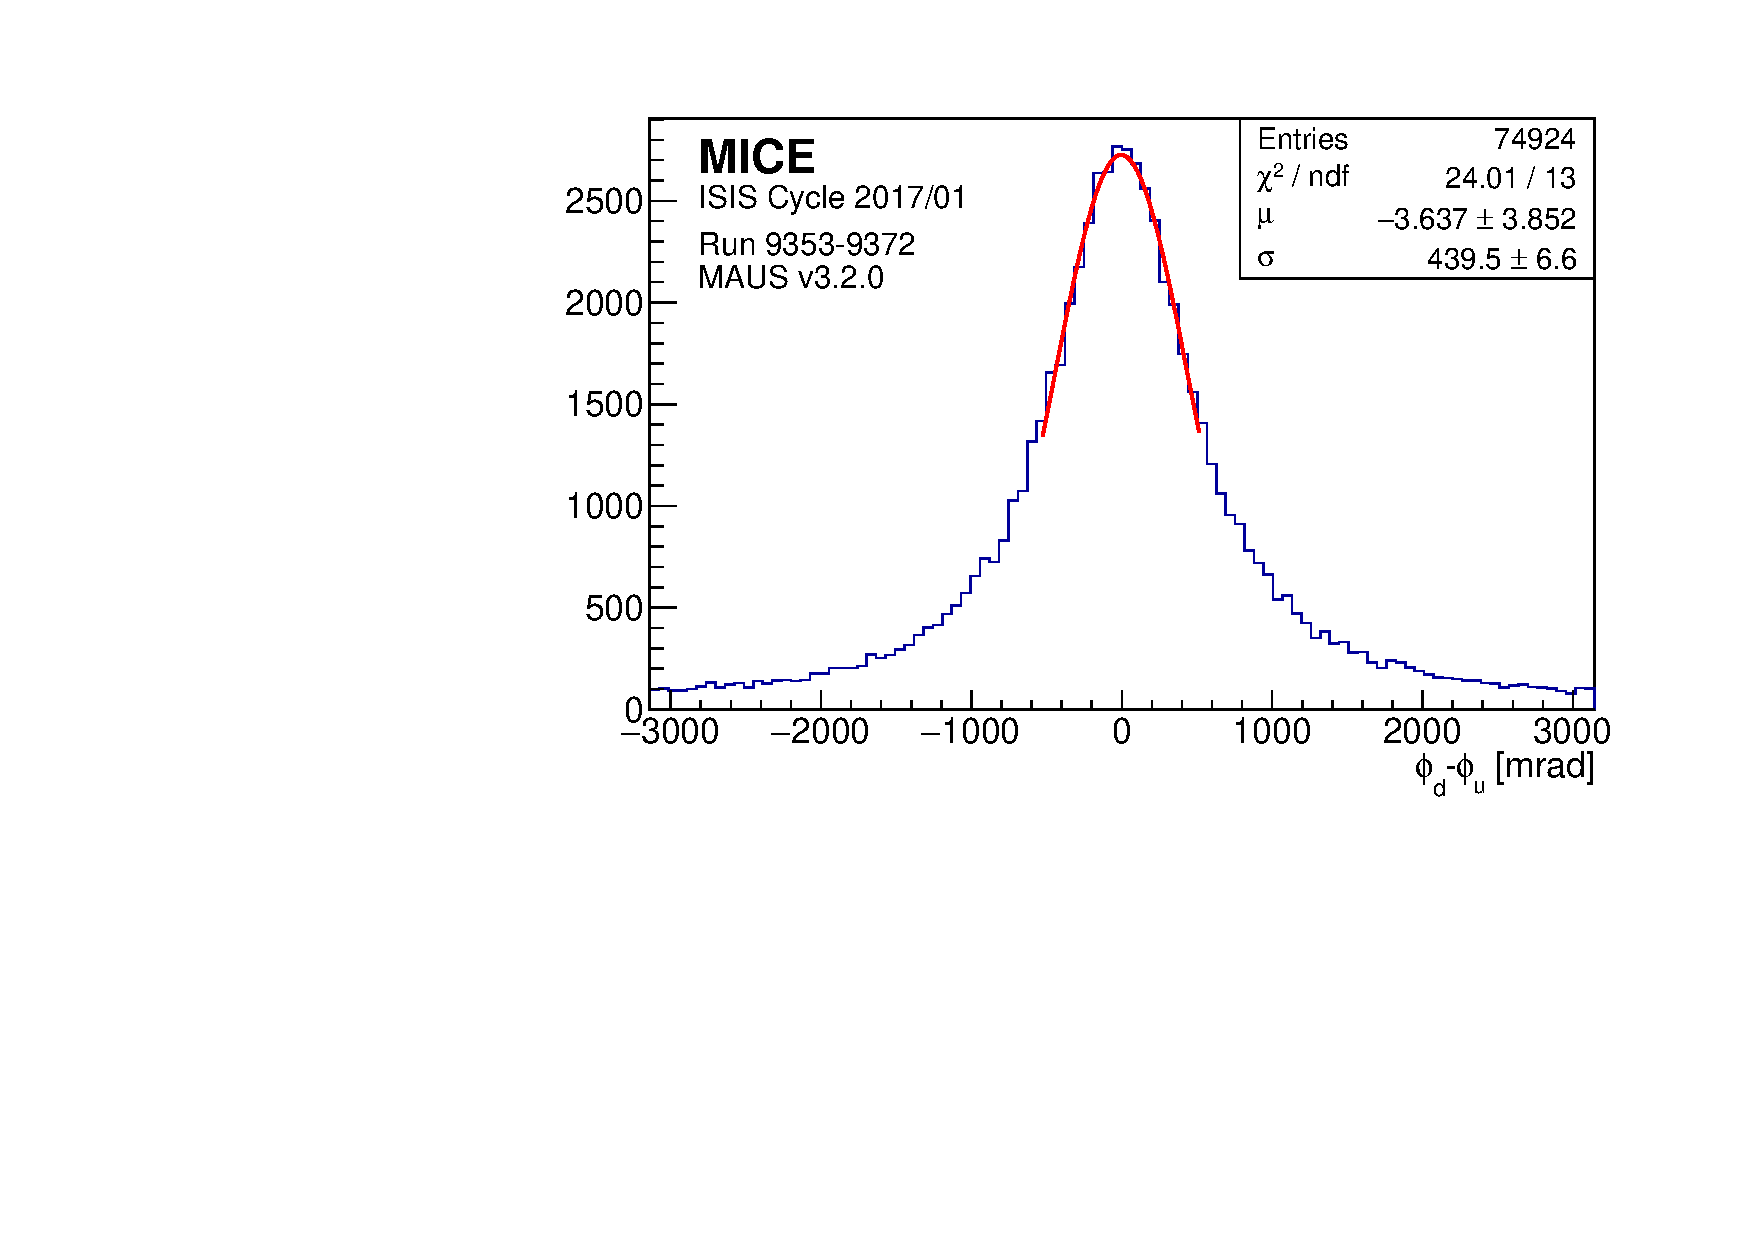
\includegraphics[width=\textwidth]{data_test/tkd_phi_res.pdf}
	\end{minipage}
	\caption{Tracker-to-tracker residual distributions in position (\textbf{top}) and angle (\textbf{bottom}).}
	\label{fig:tracker_residuals}
\end{figure}

The upstream tracker tracks are extrapolated into TOF1 and the downstream tracker tracks are propagated into the three downstream particle identification detectors: TOF2, the KL and the EMR. The residual plots are represented in figure~\ref{fig:pid_residuals}. The values obtained show good agreement between the tracks and the space points measured in other MICE detectors.

\begin{figure} [!htb]
	\centering
	\begin{minipage}[b]{.475\textwidth}
		\centering
		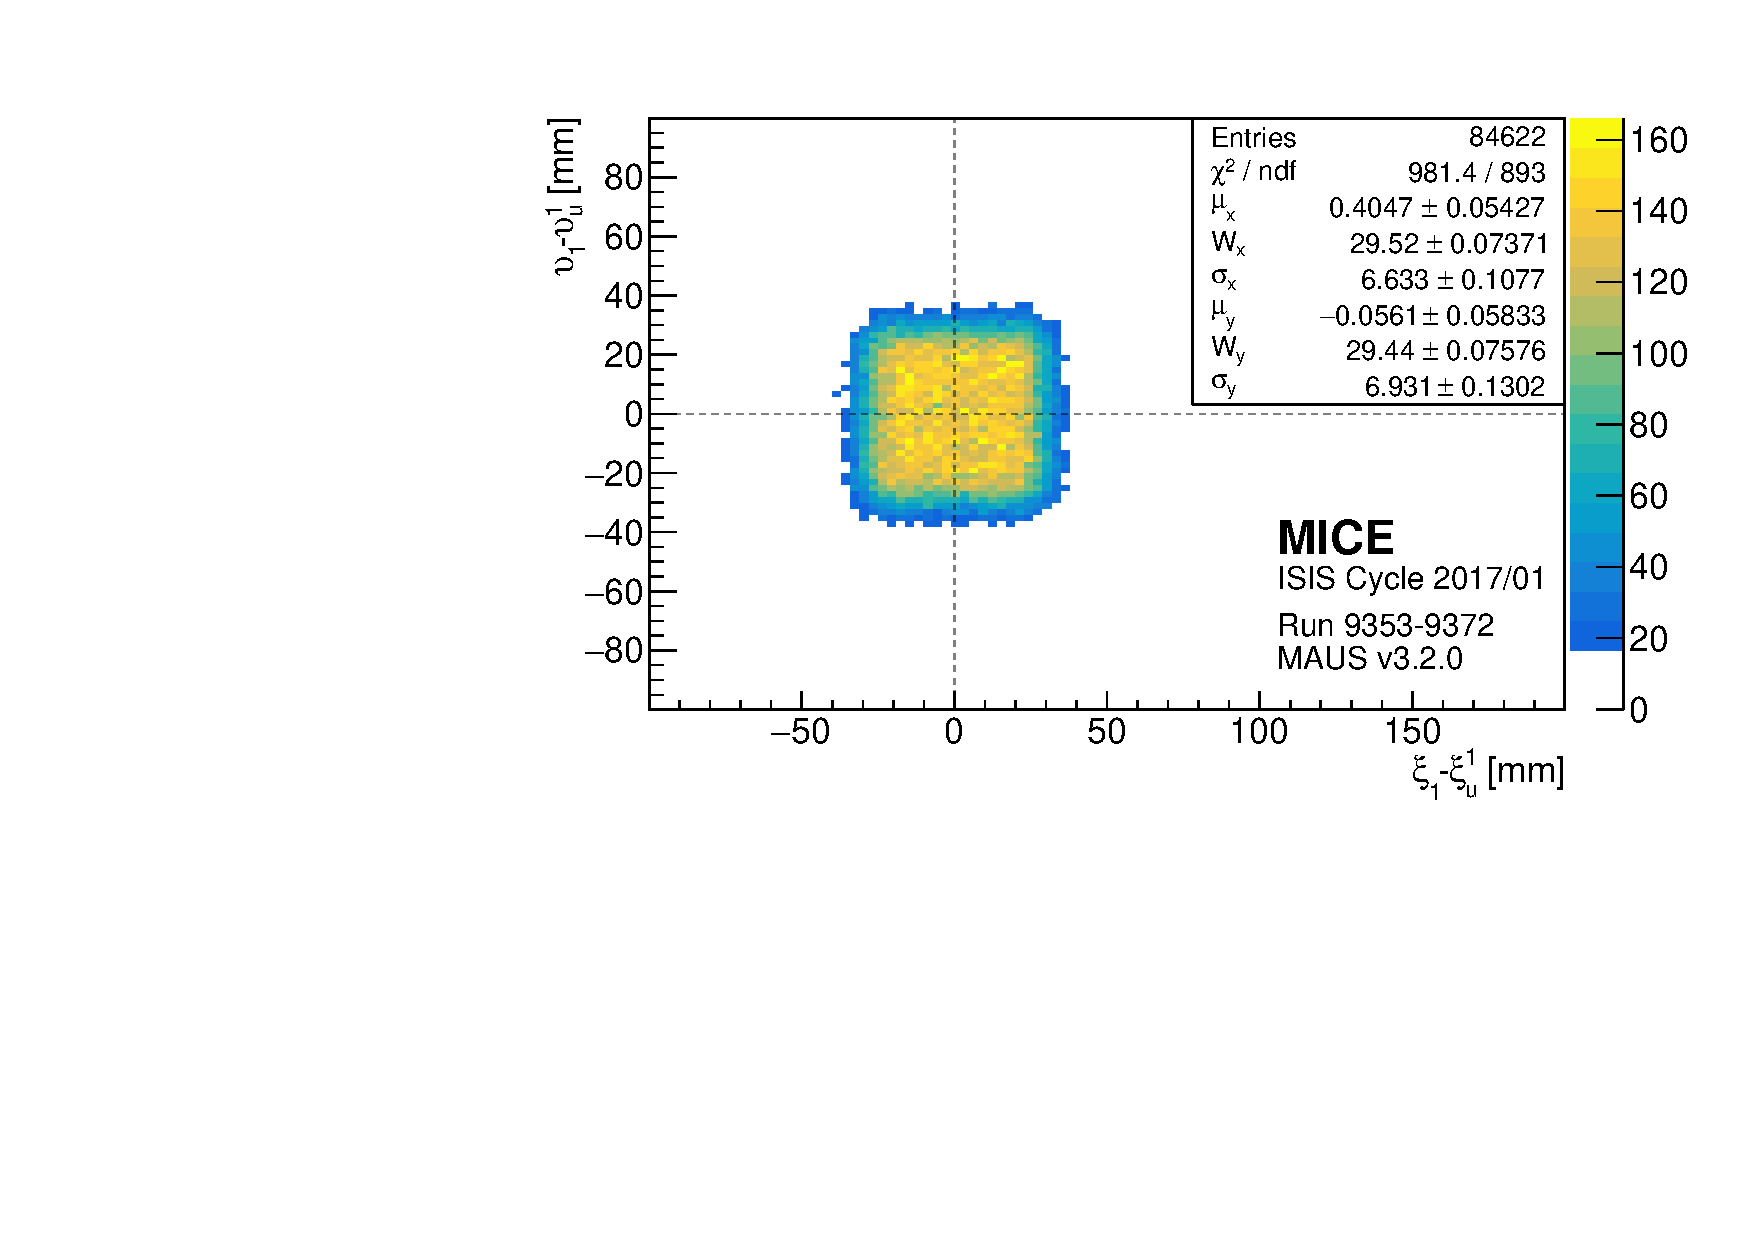
\includegraphics[width=\textwidth]{data_test/tof1_xy_res.pdf}
	\end{minipage}
	\hfill
	\begin{minipage}[b]{.475\textwidth}
		\centering
		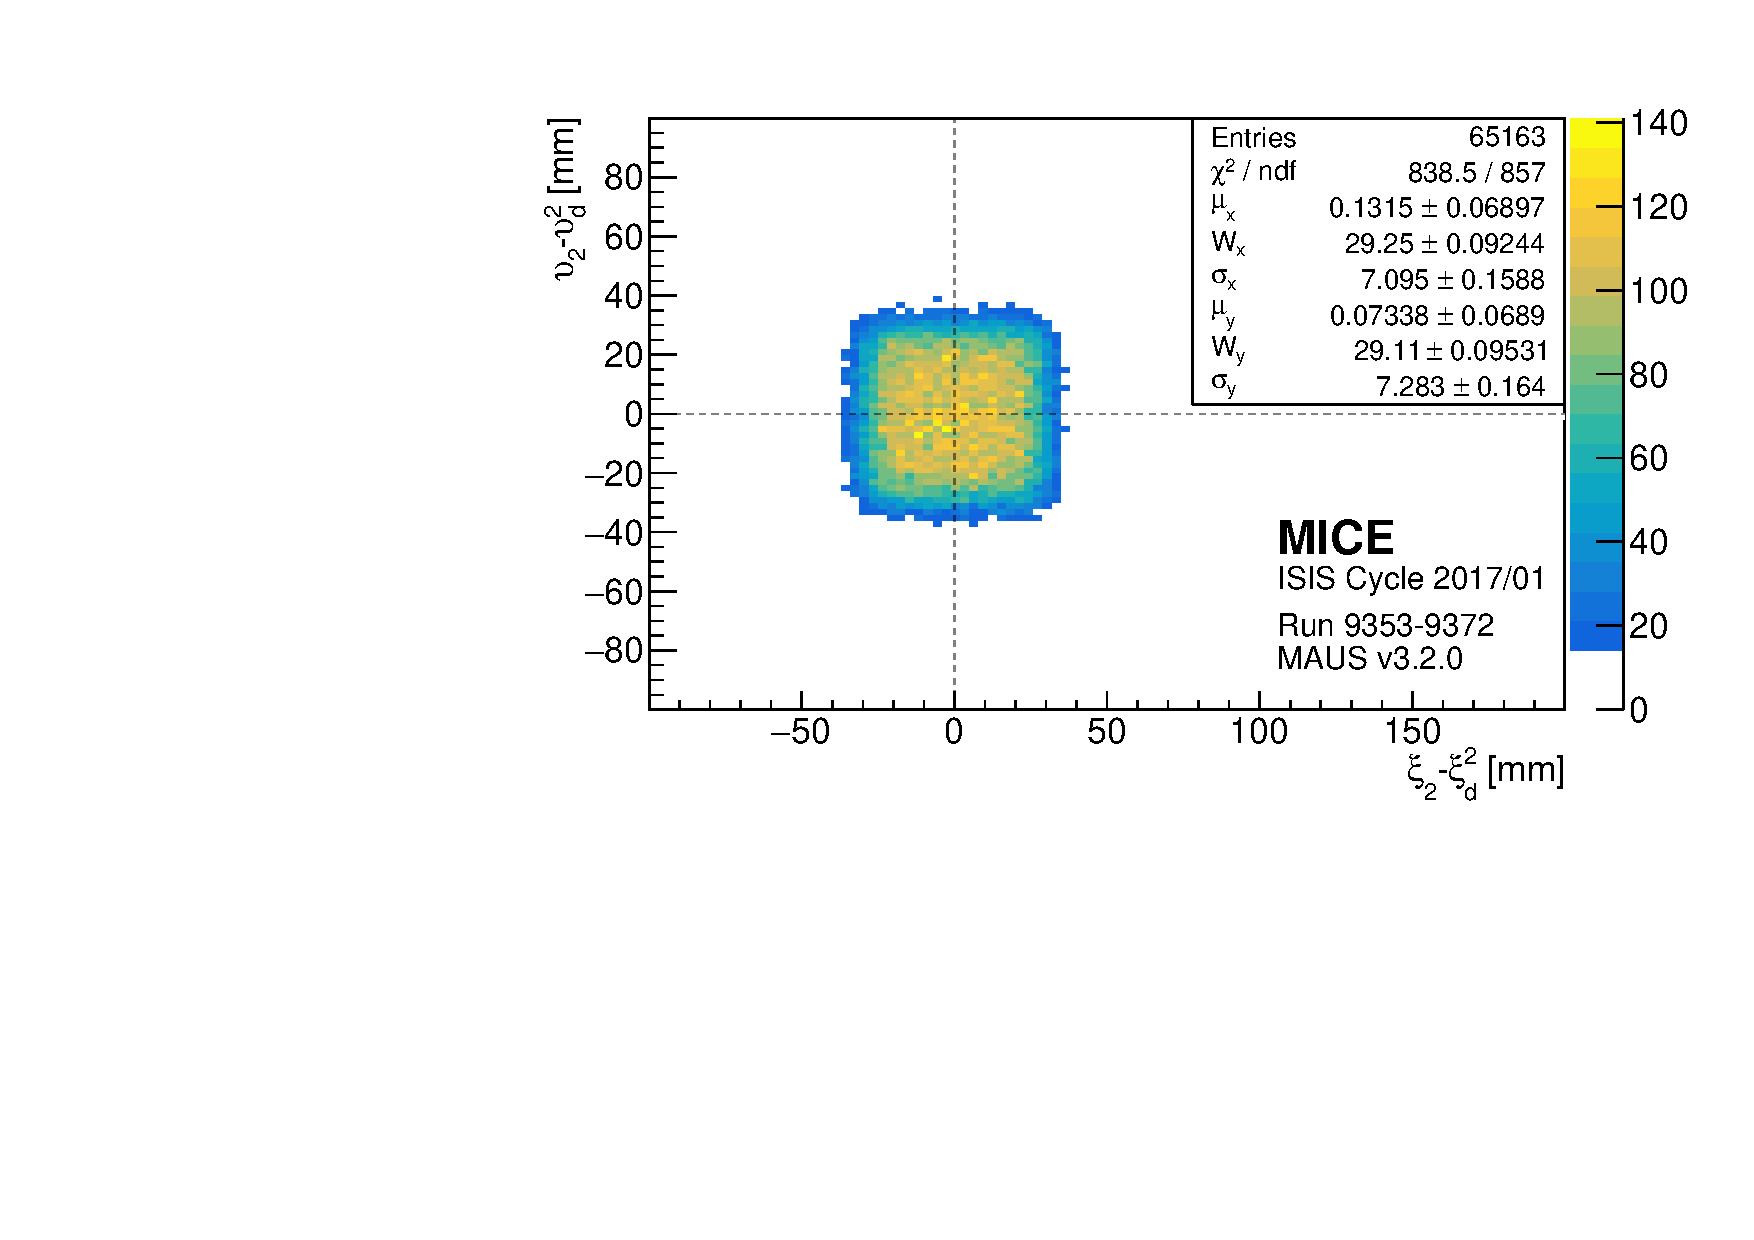
\includegraphics[width=\textwidth]{data_test/tof2_xy_res.pdf}
	\end{minipage}
	
	\begin{minipage}[b]{.475\textwidth}
		\centering
		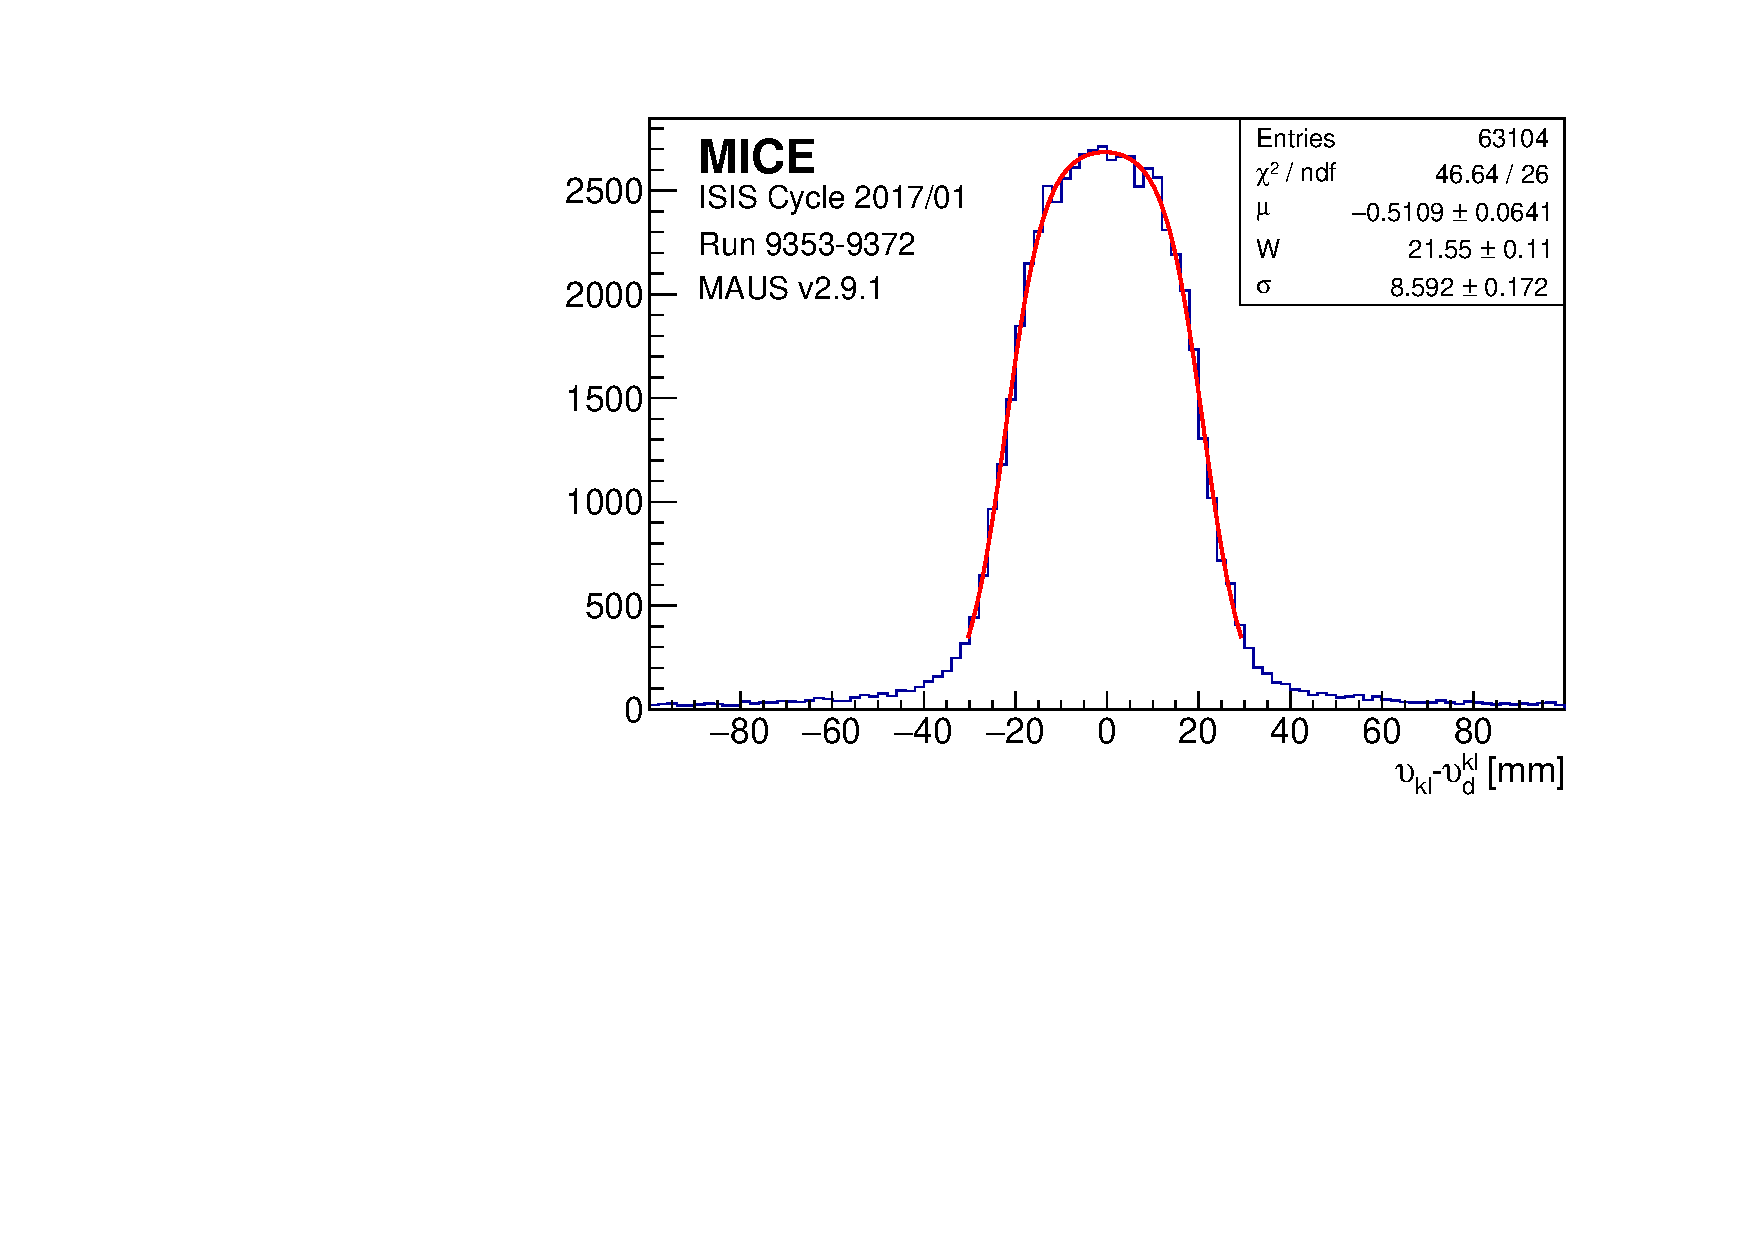
\includegraphics[width=\textwidth]{data_test/kl_y_res.pdf}
	\end{minipage}
	\hfill
	\begin{minipage}[b]{.475\textwidth}
		\centering
		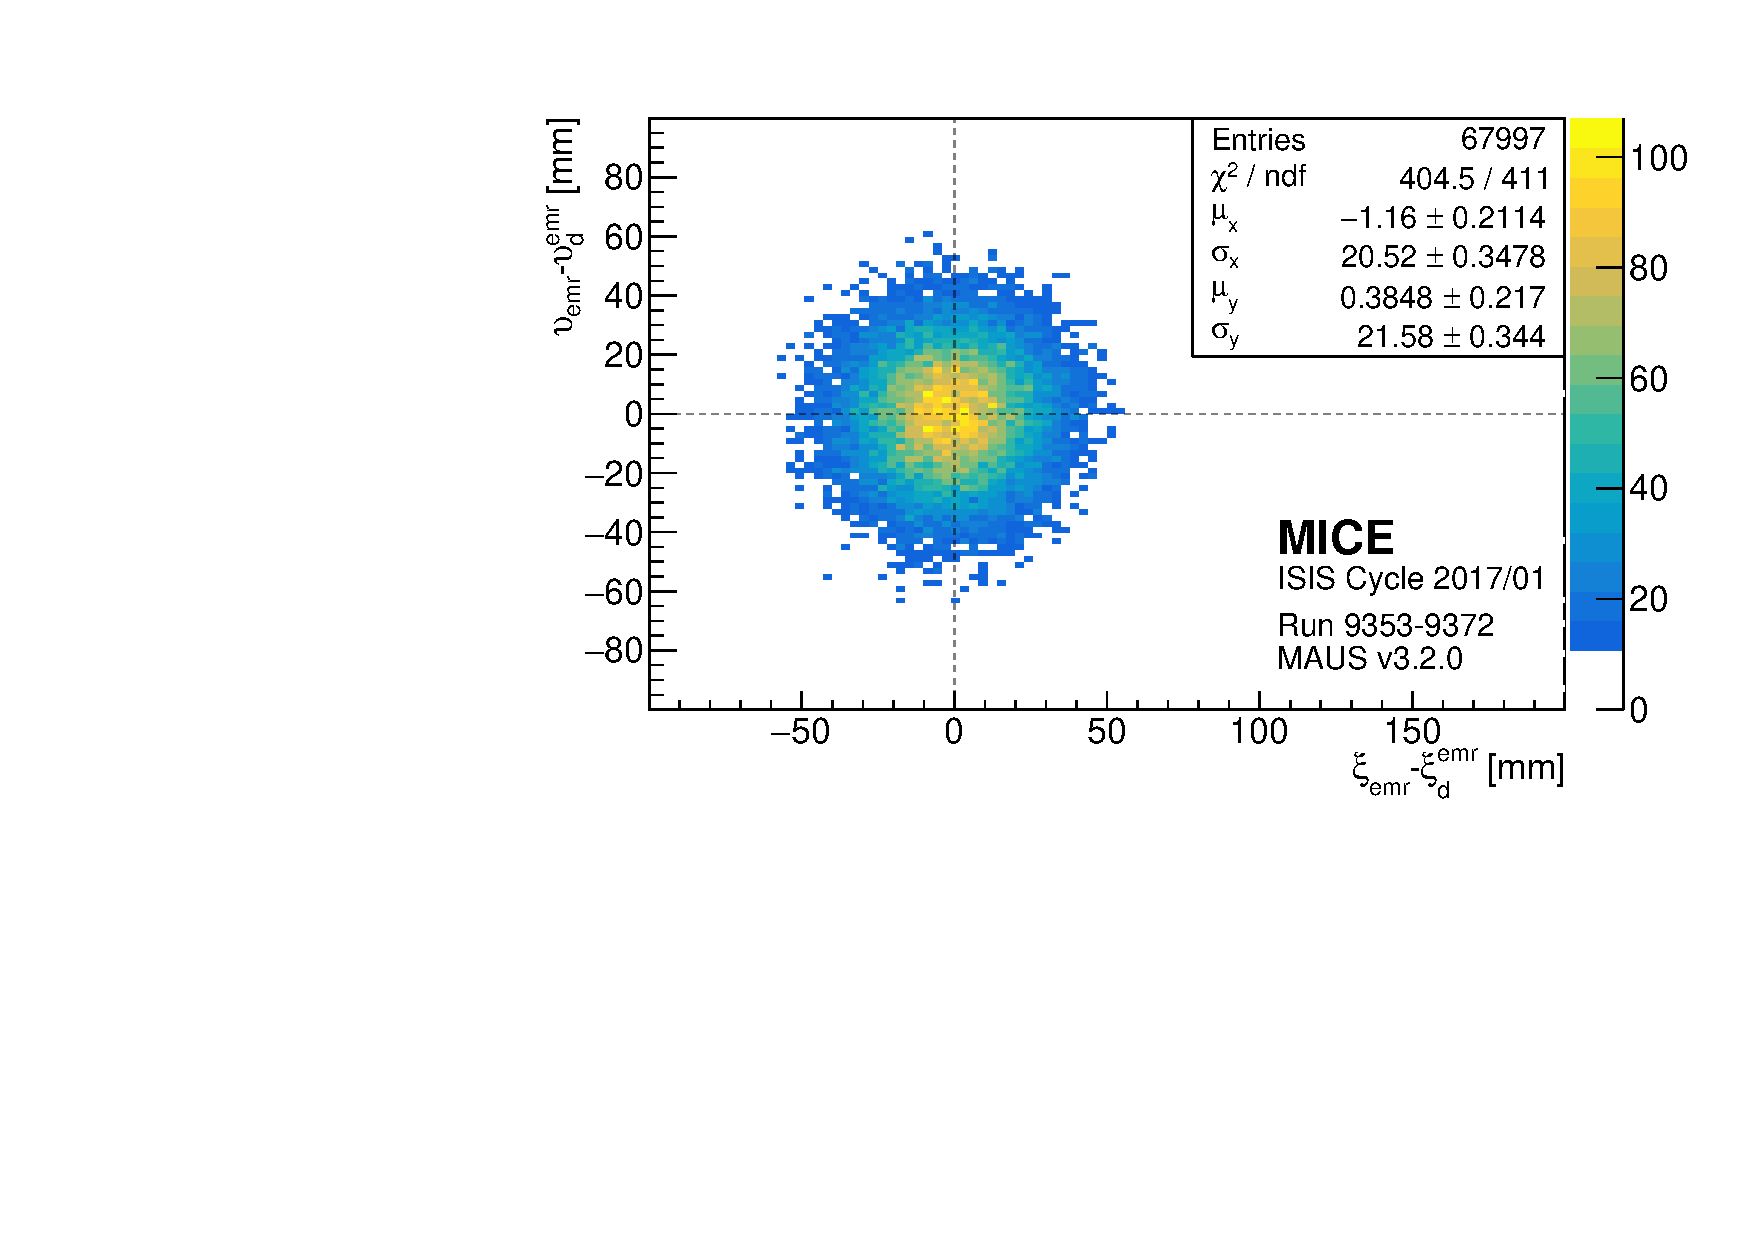
\includegraphics[width=\textwidth]{data_test/emr_xy_res.pdf}
	\end{minipage}
	\caption{Tracker to particle identification detectors residual distributions (TOF1, TOF2, KL and EMR).}
	\label{fig:pid_residuals}
\end{figure}

Special care is taken when evaluating the central value of the residual distributions. The two trackers and the Electron-Muon Ranger have a sufficient spacial resolution to follow a near-Gaussian distribution. The residuals involving these detectors are fitted with a standard multivariate normal of mean $\bm{\mu}$ and width $\bm{\sigma}$ between the two half-maximum, i.e. in the range $\bm{\mu}\pm1.1775\,\bm{\sigma}$. The TOF hodoscopes and the KL do not have a sufficient resolution to produce residuals that follow a Gaussian distribution. A probability density function of the form
\begin{equation}
h(x)=\frac{1}{4W}\left(\tanh\left[\frac{x-\mu+W}{\sigma}\right]-\tanh\left[\frac{x-\mu-W}{\sigma}\right]\right)
\end{equation}
is used in each projection to fit the residuals involving the low granularity detectors. The constant $\mu$ represents the central value of the residual distribution, $\sigma$ the residual width and $W$ the half-width of one of the low-resolution detector pixel. The parameters obtained for each of the fits are represented on the residual graphs. The values found for $W$ are consistent with pixels of 6\,cm in TOF1 and TOF2 and of 4.4\,cm in the KL.
